%\documentclass[fontsize=10pt,conference=acm, submission]{}
\documentclass[9pt,sigconf,letterpaper]{acmart}


% General
% -------
\usepackage{pdflscape}
\usepackage{xcolor}
\usepackage{comment}
\usepackage{float}
\usepackage{balance}
\usepackage{xspace}
\usepackage{subcaption}
\usepackage{multirow}
\usepackage{placeins}

\usepackage[font=small,format=plain,labelfont=bf,textfont=it]{caption}
\addtolength{\textfloatsep}{-0.15in}

\usepackage{placeins}
\usepackage{cleveref}
\hypersetup{citecolor = blue}
\usepackage[framemethod=TikZ]{mdframed}
\usepackage[utf8]{inputenc}
\graphicspath{{figures/}}

\makeatletter
\def\input@path{{sections/}{./}}
\makeatother


\crefformat{section}{\S#2\color{blue}#1#3} % see manual of cleveref, section 8.2.1
\crefformat{subsection}{\S#2\color{blue}#1#3}
\crefformat{subsubsection}{\S#2#1#3}

%\setcopyright{none}
%\settopmatter{printacmref=false} % Removes citation information below abstract
%\renewcommand\footnotetextcopyrightpermission[1]{} % removes footnote with conference information in first column
%\pagestyle{plain} % removes running headers


%%% Adding new line after subsubsection
\makeatletter
\def\subsubsection{\@startsection{subsubsection}{3}%
  \z@{.5\linespacing\@plus.7\linespacing}{.1\linespacing}%
    {\normalfont\itshape}}
    \makeatother





% Bibliography
% ------------
%\bibliography{paper}

% Commands
% --------

\pgfsetarrows{latex-latex}
\tikzset{%
  base/.style = {inner sep=5pt,
                 text centered,
                 thin,
                 font=\rmfamily},
  round/.style = {base,
                  rectangle,
                  rounded corners=1ex,
                  draw=black,
                  fill=gray!20,
                  minimum height=0.35in}
}

%%%%%%%%%% MACRO NAMES %%%%%% 
\newcommand{\teams}{Teams\xspace}
\newcommand{\meet}{Meet\xspace}
\newcommand{\zoom}{Zoom\xspace}
\newcommand{\zoomnative}{Zoom-native\xspace}
\newcommand{\zoombrowser}{Zoom-Chrome\xspace}
\newcommand{\teamsnative}{Teams-native\xspace}
\newcommand{\teamsbrowser}{Teams-Chrome\xspace}

\newcommand{\tarun}[1]{[\textcolor{blue}{\textit{Tarun: #1}}]}
\newcommand{\jamie}[1]{[\footnote{\textcolor{red}{\textit{Jamie: #1}}]}}
\newcommand{\kyle}[1]{[\textcolor{green}{\textit{Kyle: #1}}]}

%\usepackage[table]{xcolor}
\definecolor{ps0}{rgb}{0.97, 0.98, 1.00}
\definecolor{ps1}{rgb}{0.78, 0.86, 0.94}
\definecolor{ps2}{rgb}{0.42, 0.68, 0.84}
\definecolor{ps3}{rgb}{0.13, 0.44, 0.71}
\definecolor{ps4}{rgb}{0.03, 0.19, 0.42}
\newcommand{\cbssss}[1]{\cellcolor{ps4}  \textcolor{white}{#1}}
\newcommand{\cbsss}[1]{\cellcolor{ps3}  \textcolor{white}{#1}}
\newcommand{\cbss}[1]{\cellcolor{ps2} #1}
\newcommand{\cbs}[1]{\cellcolor{ps1} #1}
\newcommand{\cb}[1]{\cellcolor{ps0} #1}


%\newcommand{\rev}[2]{\sout{#1}\textcolor{blue}{#2}}
%Accept revisions
\newcommand{\rev}[2]{{#2}}


%%%%%%%%%%%%%%%%%%%%  SPACE SAVINGS %%%%%%%%%%%%%%%%%%%%%%

\usepackage[all=normal,wordspacing]{savetrees}
%\setlist[itemize]{leftmargin=*}
\usepackage[normalem]{ulem}

\copyrightyear{2021}
\acmYear{2021}
\acmConference[IMC '21]{Internet Measurement Conference}{November 2--4, 2021}{Virtual Event}
\acmBooktitle{Internet Measurement Conference (IMC '21), November 2--4, 2021, Virtual Event}
\acmPrice{TBA}
\acmDOI{10.1145/3487552.3487842}
\acmISBN{978-1-4503-9129-0/21/11}

%%%%%%%%%%%%%%%%%%%%  TITLE/AUTHORS  %%%%%%%%%%%%%%%%%%%%%

\title{Measuring the Performance and Network Utilization of Popular Video Conferencing Applications}


\author{Kyle MacMillan, Tarun Mangla, James Saxon, Nick Feamster}
%\orcid{0000-0002-5151-4517}
\affiliation{%
  \institution{Department of Computer Science, University of Chicago}
  \streetaddress{5730 South Ellis Ave}
  \city{Chicago}
  \state{IL}
  \postcode{60637}
  \country{USA}}
\email{{macmillan,tmangla,jsaxon,feamster}@uchicago.edu}


%\titlespacing\section{0pt}{*1.8}{*1.1}
%\titlespacing\subsection{0pt}{*1.5}{*1.1}
%\titlespacing\subsection{0pt}{*1.3}{*0.8}

\renewcommand{\paragraph}[1]{\vspace*{0.03in}\noindent\textbf{#1}}

%%%%%%%%%%%%%%%%%%%%  START OF DOCUMENT  %%%%%%%%%%%%%%%%%

\begin{document}

\begin{sloppypar}
\abstract{
Video conferencing applications (VCAs) have become a critical Internet
application, even more so during the COVID-19 pandemic, as users worldwide now rely on them for
work, school, and telehealth. % COVID-19 has spurred unprecedented
%growth in the use of VCAs, with some Internet service providers seeing
%video conferencing traffic triple over an eight-month period
%in 2020. 
It is important to understand the resource requirements of different
VCAs and how these VCAs perform under different network conditions, including:
how much ``speed'' (specifically, upstream and downstream throughput) a VCA needs to support high quality of experience, how
VCAs perform under temporary reductions in available capacity; how they compete
with themselves, with each other, and with
other applications; and how usage modality (e.g., number of participants)
affects utilization.  We study three modern VCAs: Zoom, Google Meet,
and Microsoft Teams.   Answers to these questions differ substantially
depending on VCA.  First, the average utilization on an unconstrained
link varies between 0.8~Mbps and 1.9 Mbps.  Given temporary reduction of
capacity, some VCAs can take as long as 45 seconds to recover to average.  Differences in proprietary
congestion control also create unfair bandwidth allocations: in
constrained bandwidth settings, one Zoom video conference can consume more than 75\%
of the available bandwidth when competing with another VCA (e.g., Meet, Teams).  For some VCAs, client utilization can
decrease as the number of participants increases, due to the reduced video
resolution of each participant's video stream given a larger number of
participants. 
}



% Video conferencing has been one of the killer applications of the Internet. The video conferencing application (VCA) landscape has recently undergone significant change owing to the ongoing covid pandemic with the introduction of new VCA applications (e.g., Google Meet, Microsoft Teams) or revamping of incumbent VCA (e.g., Zoom, Bluejeans) to facilitate user engagement. The VCAs, however, have differed in their design choices and features. Understanding these differences with their impact on application performance and network consumptions can help in improving the design of future VCAs.  

% In this paper, we conduct extensive measurments contrasting the design differences for three popular VCAs, namely Zoom, Google Meet, and Microsoft Teams. We first study the application performance metrics in a 2-person call under different network conditions. We find that differences in application performance under same network conditions which can be attributed to differences in encoding mechanisms, application-level capping, bandwidth estimation techniques. We also found that performance varies across device platform even for the same application (e.g., native client better than the web client). We next study the impact of usage modality (e.g., gallery vs speaker mode in zoom) on network consumption and find some interesting differences in network consumption based on the usage modality. For instance, Zoom typically increases the sent video resolution of the user under speaker mode. Finally, we also study how different VCAs share bandwidth with other applications (file download, video streaming, and other VCAs) in terms of fairness. We find interesting differences wherein we find that applications do not share bandwidth fairly with other internet applications. 
% %A systematic understanding of the VCA design and its implications on network-levek performance is can be useful especially for improving the design of these services. In this paper, we conduct extensive measurements to understand and contrast the design of three popular VCAs, namely Zoom, Google Meet, and Microsoft Teams. 



%The video conferencing application (VCA) landscape has changed significantly because of COVID-19, with the introduction of new VCAs (e.g. Google Meet, Microsoft Teams) and renewal of incumbent VCAs (e.g. Zoom, Bluejeans). Because these VCAs differ in their design choices and features, it is critical that we understand how these differences impact application performance and network consumption under different network conditions and call modalities. This has two-fold advantages: i) a comparative analysis can uncover best design practices useful for improving current and future VCAs, and ii) understanding VCA network consumption for different contexts can be useful for ISPs in network provisioning and for telecommunication policy makers in defining benchmarks for Broadband access.   




%We find differences in VCA behavior under same static network conditions, such as different maximum (or nominal) bitrate (0.8 Mbps-1.9 Mbps) and inefficient network utilization for some VCAs under constrained links (e.g., 50\% for Meet). Next, we study how each VCA responds to dynamic network conditions by introducing (1) temporary bandwidth drops or (2) a competing application (e.g. Netflix, TCP iPerf3) on the same link. All require at least 20 seconds to return to their nominal sending rate following a temporary uplink constraint to 0.25Mbps. Further, Microsoft Teams is especially slow to recover from drop in downlink bandwidth because they do not do congestion control from the cloud. When competing with other applications on a constrained link, Zoom aggressively consumes available bandwidth, while Meet and Teams back off at low bandwidths. Finally, we investigate how usage modality (e.g. number of participants, speaker vs. gallery mode) affect consumption. Increasing the number of participants may reduce a user's network utilization. We find that a user's sending bitrate at least doubles when their video is pinned by all other participants. 

%All VCAs require at least 20 seconds to return to their nominal sending rate following a temporary uplink constraint to 0.25Mbps. Further, Microsoft Teams is especially slow to recover from drop in downlink bandwidth because they do not do congestion control from the cloud. When competing with other applications on a constrained link, Zoom aggressively can consume over 75\% of the available bandwidth when competing with Meet and Teams. 


\begin{CCSXML}
<ccs2012>
<concept>
<concept_id>10002951.10003227.10003251.10003255</concept_id>
<concept_desc>Information systems~Multimedia streaming</concept_desc>
<concept_significance>500</concept_significance>
</concept>
<concept>
<concept_id>10003033.10003079.10011704</concept_id>
<concept_desc>Networks~Network measurement</concept_desc>
<concept_significance>500</concept_significance>
</concept>
</ccs2012>
\end{CCSXML}

\ccsdesc[500]{Networks~Network measurement}
\ccsdesc[500]{Information systems~Multimedia streaming}

\keywords{Video conferencing, Network measurements, Real-time Streaming, QoE}

\maketitle

\section{Introduction}\label{sec:intro}
COVID-19 has made video conferencing applications (VCAs) both common and necessary. People now regularly use VCAs for work, school, and telehealth, as activities have shifted from in-person to online. The success of remote communication indicates that VCAs will continue to play a critical role during and after the pandemic. However, VCAs are unique among internet applications and their increased use has altered the makeup of internet traffic. 

VCAs differ from other popular types of internet activity in several ways. Most notably, VCAs have far greater uplink utilization. Video streaming and internet browsing, two dominant sources of internet traffic, [receive the bulk of their traffic and send very little]. VCAs, however, send a video stream on the uplink. Further, VCAs do not benefit from network optimizations used in video streaming. Video streaming applications can "buffer" by fetching video ahead of time, then sporadically downloading when necessary. VCAs can not download video ahead of time because the video occurs in real-time. As a result, VCAs require a consistent and low-latency connection.

The earliest studies on VCAs focused on Skype, the dominant application in the VCA landscape at the time. These works sought to understand Skype from both a design and performance perspective. As the VCA landscape evolved over time, later work shifted their attention to newer VCAs and the protocols they used. 

While significant research and measurement studies have been conducted on VCAs in the past, both the VCAs and how we use them has since changed. Several new VCAs (e.g. Microsoft Teams, Google Meet) have been introduced, while existing VCAs (e.g. Zoom) have undergone a renewal. In light of these developments, it is important to investigate how differing VCA design choices impact application performance and network consumption. 


The continuing reliance on VCAs makes understanding these network requirements precisely crucial. In this paper, we conduct a comparative analysis of three popular VCAs: Google Meet, Microsoft Teams, and Zoom. We can determine these requirements by measuring VCA performance and consumption under realistic network conditions, including low bandwidth availability and other activity on the same network. Our goal is to understand the following:
\begin{enumerate}
    \item How VCAs performance varies under different static network conditions.
    \item How VCAs respond to temporary drops in bandwidth availability.
    \item How VCAs interact with competing applications on a constrained link.
    \item How usage modalities (number of participants, speaker vs. gallery viewing) affect network consumption.
\end{enumerate}

Answering the first question gives us insight into the minimum network requirements for each VCAs. 




% \begin{itemize}
% \item VCAs have been touted as a killer application for the Internet connecting millions of users. Significant research and measurement studies have been conducted benchmarking the VCAs of the time, their design choices and its impact on application performance. 

% \item The VCA application has undergone significant change in the covid-era of work from home/school with either new VCAs have been introduced or existing applications significantly revamped.

% \item In the context of these changes, it is important to revist the earlier measurement studies especially understanding how these changes relate to application performance and network consumption.

% \item In this paper we do a comparative analysis of three popular applications, namely zoom, meets, and teams. 

% \item Our analysis compares the VCAs along these three questions: i) How does the application performance vary under different network conditions?, ii) What is the impact of different VCA usage modality on network consumption, iii) Are the VCA applications fair in terms of bandwidth sharing when compared to other applications or transport protocols.

% \item Underlying question: what network conditions are required to support multiple streams through a link, at full performance?  Conversely, what network conditions are associated with degraded performance?  (Implications for broadband debates.)

% \item Insights: We find that ... 
% \end{itemize}

\section{Background \& Experiment Setup}
\label{sec:background}

We provide a brief background on video conferencing transport, technology, and
architecture before turning to our experiment setup.

\subsection{Video Conferencing Applications}

Most modern VCAs use Real-time Transport Protocol (RTP)~\cite{schulzrinne1996rtp,
schulzrinne2003rfc3550} or its variants~\cite{baugher2004secure, zoom_rtp} to
transmit media content. The audio and video data is generally transmitted over
separate RTP connections. RTP also uses two other protocols in conjunction,
Session Initiation Protocol (SIP)~\cite{rosenberg2002sip} to establish
connection between clients and RTP Control Protocol
(RTCP)~\cite{schulzrinne2003rfc3550} to share performance statistics and
control information during a call. Despite using well-known protocols, VCAs
can differ from each other significantly across the following dimensions:


\begin{itemize}
    \itemsep=-1pt
    \item \textbf{Network mechanisms}: RTP and the associated protocols are
        implemented in the application-layer. Thus, the specific
        implementation of the protocols can vary across VCAs. For instance,
        Zoom reportedly uses a custom extension of RTP~\cite{zoom_rtp}).
        Furthermore, the key network functions, i.e., congestion control and
        error recovery, can also be different and proprietary. 

    \item \textbf{Application-layer parameters}: These include media encoding
        standards and default bitrates. More recent video codecs (e.g., VP9,
        H.264) can encode at the same video quality with fewer bytes when
        compared to older codec (e.g., VP8), albeit with a higher compute
        overhead~\cite{bienik2016performance}. 
    
    \item \textbf{Streaming architecture}: VCAs can either choose to use
        direct connections or use relay servers. Centralized servers are
        almost always used for multi-point calls to combine data from multiple
        users. VCAs can differ in the exact strategies of data combination as
        well as the geographic footprint of their servers. For instance, Zoom
        rapidly expanded its server infrastructure to support increased call
        volume because of COVID-19~\cite{liu2020characterizing}. 

\end{itemize}
\noindent
Differences across one or more of these factors can lead to different VCA
network utilization and performance. In this paper, we aim to dig deeper into
some of these differences for a subset of VCAs. 


\subsection{Experiment Setup} 
\label{subsec:setup}

\paragraph{Video Conferencing Applications}:
In this paper, we study three popular VCAs---\zoom, Google \meet, and Microsoft \teams.
These VCAs have been used extensively worldwide over the past year, especially
in enterprises and educational institutions~\cite{vca_share}.  Teams and Zoom
provide desktop applications as well as browser clients, whereas Meet is ``native"
in the Chrome. Most of our tests are conducted using the desktop
applications for Teams and Zoom, and using the Google Chrome browser for Meet.
In-browser tests for Teams and Zoom are specified by \textit{\teamsbrowser}
and \textit{\zoombrowser}, respectively. We use Chrome (Meet) version
89.0.4389, Zoom client version 5.6.1, and Teams client version 1.4.00.7556.


\paragraph{Laboratory Environment}:
We conduct experiments in a controlled environment.  We begin by describing our experimental setup for a 2-party call. We use two identical laptops, referred to as C1 and C2, representing the two VCA clients. Each laptop is a Dell Latitude 3300 with a screen resolution of 1366 $\times$
768 pixels and running Ubuntu 20.04.1. The laptops have a wired connection to
a Turris Omnia 2020 router and access a dedicated 1~Gbps symmetric link
to the Internet.  Each experiment consists of a call between C1 and C2 under a
pre-specified network bandwidth profile and VCA. The bandwidth profile is
emulated by shaping the link between C1 and the router using traffic control
(\texttt{tc}). A pre-recorded talking-head video\footnote{It would be inappropriate to use the 
device webcam as the video, because without movement, VCAs compress the video
and ultimately send at a much lower rate than during a normal call.} with a
resolution of 1280 $\times$ 720 is used as the video source for the call, using \texttt{ffmpeg}.
This is done to both replicate a real video call and ensure consistency across
experiments. All experiments are conducted with the laptop lid open and the
application window maximized. 

\begin{figure*}[t!]
\begin{subfigure}[t]{0.33\textwidth}
    \centering
    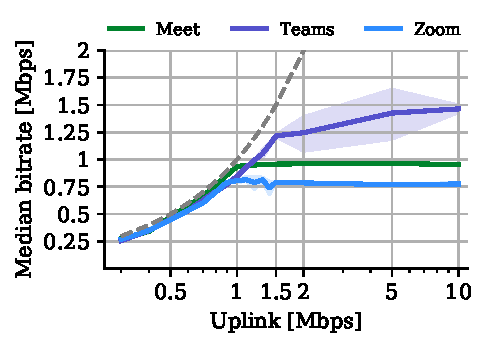
\includegraphics[width=\textwidth,keepaspectratio]{figures/static/uplink.pdf}
    \caption{Uplink bandwidth vs network bitrate %\jamie{label $x = y$}
    }
	\label{subfig:uplink_bitrate}
\end{subfigure}\hfill
\begin{subfigure}[t]{0.33\textwidth}
\centering
    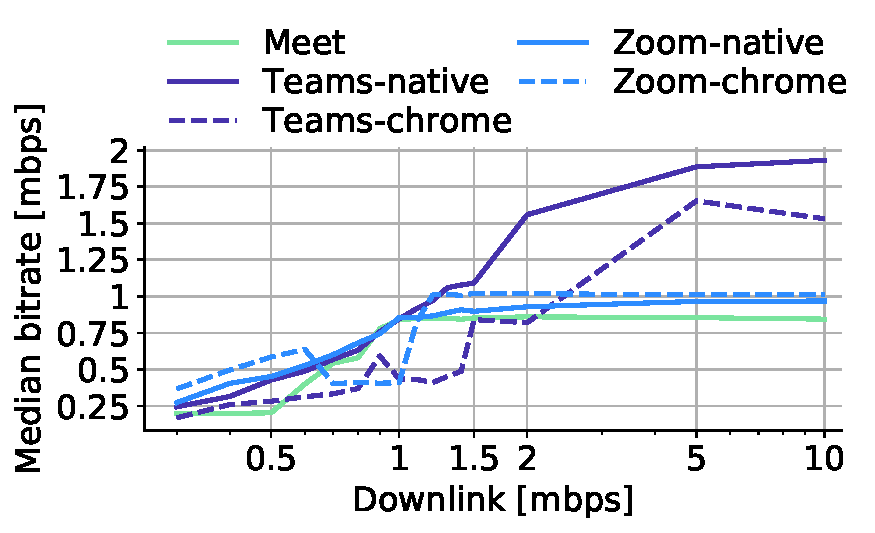
\includegraphics[width=\textwidth,keepaspectratio]{figures/static/downlink.pdf}
    \caption{Downlink bandwidth vs network bitrate}
	\label{subfig:downlink_bitrate}
\end{subfigure} \hfill
\begin{subfigure}[t]{0.33\textwidth}
\centering
    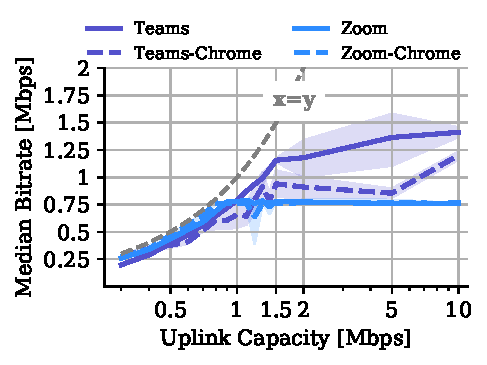
\includegraphics[width=\textwidth,keepaspectratio]{figures/static/uplink_browser.pdf}
    \caption{Impact of VCA platform %\jamie{capitalize Chrome}
    }
	\label{subfig:uplink_browser}
\end{subfigure} 
\vspace{-1em}
\caption{Utilization under different shaping levels. The bands represent 90\% confidence intervals.}
\label{fig:static}
\end{figure*}
%on the laptop and router for uplink and downlink shaping, respectively. During the competition experiments, all shaping occurs at the router.

\paragraph{Automating Experiments}: To conduct experiments at scale, we
automated the entire in-call process. We take several steps to recreate the
in-call process.  We use the Python PyAutoGUI package~\cite{pyautogui} to
automate joining and leaving calls. The package enables to programmatically
control the keyboard and the mouse by specifying coordinates or visual
elements on the screen. For \zoombrowser, we encountered CAPTCHA before
joining a call on the default browser. Using the Selenium-based Chrome
browser~\cite{selenium}, however, enabled us to bypass the CAPTCHA. Note the
experiments using Selenium are run exactly as it would be in default Chrome
browser. The workflow is controlled from C1, with TCP sockets used to
coordinate between C1 and C2.  We modify this setup slightly for subsequent
experiments (e.g., multi-party calls); those slight modifications are
described in the respective sections.


%%%%%%%%%%%%%%%%%



\begin{comment}
\paragraph{Performance metrics}: We mainly focus on the following application metrics. 
\begin{itemize}
    \item \textbf{Network bitrate}
    \item Video resolution
    \item Frames per second
    \item Freeze count
    \item Freeze duration
    \item Jitter-buffer delay 
\end{itemize}

Most of our analysis is using network bitrate. We consider other application performance metrics when they can be extracted from Google Chrome\footnote{chrome://webrtc-internals}. Our analysis shows that there is a strong correlation between network bitrate and application performance. This is intuitive as real-time streaming is characterized by low latency and thus any network interruptions usually lead to degradation in application performance. 


\subsection{Measurement Method}
  
The measurement setup consists of several components:

Hardware
\begin{itemize}
    \item matched laptops for nominal flows
          \begin{itemize}
              \item All Linux; caveats -- may not be the most-maintained apps
              \item What laptops, for the many-laptop tests?
          \end{itemize}
    \item turris router for control of single shaped link
    \item private iperf server on university network
\end{itemize}

\begin{itemize}
    \item traffic control scripts
    \item autogui; selenium for browser
          \begin{itemize}
              \item Important that we have the screen up -- see e.g., the tweet, but maybe chase the paper, about the struggle of getting the machines to actually render flows being important.
              \item client vs browser
              \item sw versions?
          \end{itemize}
    \item pcap, iperf logs
    \item webrtc
          \begin{itemize}
              \item difference between meet and zoom 
          \end{itemize}
    \item Zoom API access (\& limitations?)
    \item control over sockets?
\end{itemize}

\begin{table*}[t!]
\centering
\begin{tabular}{|c|c|c|c|c|}
\hline
\paragraph{VCA} & \textbf{Platforms}     & \textbf{Encoding} & \textbf{Direct connection?} & \textbf{Network Protocol} \\ \hline
\hline 
Meet  & Browser, Phone         & VP9/VP8   & No                 & RTP (WebRTC)     \\ \hline
Teams & Native, Browser, Phone & VP9       & ?                  & RTP              \\ \hline
Zoom  & Native, Browser, Phone & H.264 SVC & Yes                & Variation of RTP \\ \hline
\end{tabular}
\caption{Design parameters of selected VCAs}
\label{tab:vca_overview}
\end{table*}
\end{comment}


\begin{figure}[t]
\vspace{-7em}
\begin{subfigure}[t]{0.45\textwidth}
    \centering
    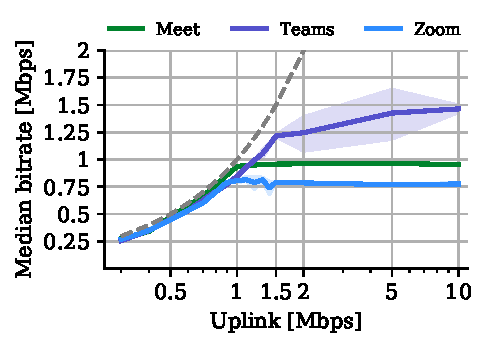
\includegraphics[width=\textwidth,keepaspectratio]{figures/static/uplink.pdf}
    \caption{Uplink bandwidth vs network bitrate}
	\label{subfig:uplink_bitrate}
\end{subfigure}
\begin{subfigure}[t]{0.45\textwidth}
\centering
    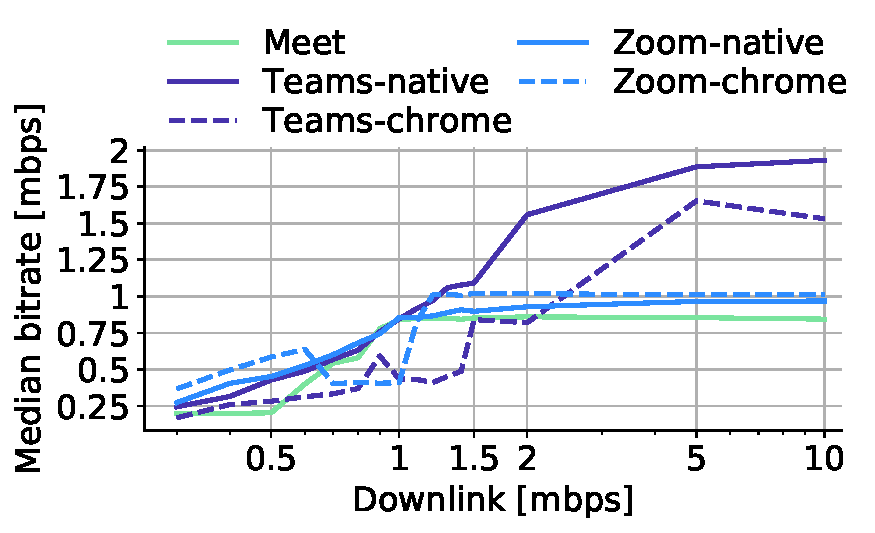
\includegraphics[width=\textwidth,keepaspectratio]{figures/static/downlink.pdf}
    \caption{Downlink bandwidth vs network bitrate}
	\label{subfig:downlink_bitrate}
\end{subfigure} 
\caption{Utilization under different link capacities}
\label{fig:static}
\end{figure}

\section{Static Network Conditions}\label{sec:static}

\begin{figure*}[]
	%\vspace{-10em}
    \begin{subfigure}[t]{0.3\textwidth}      
    		\centering
        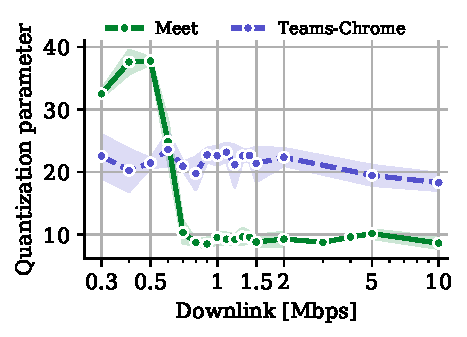
\includegraphics[width=\textwidth,keepaspectratio]{figures/static/downlink_r_qpsum.pdf}
        \vspace{-2em}
        \caption{Quantization parameter}
 		\label{subfig:downlink_video_bitrate}
    \end{subfigure}%
    \hfill
	\begin{subfigure}[t]{0.3\textwidth}   
        \centering
        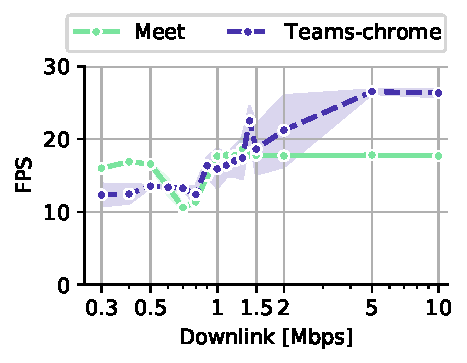
\includegraphics[width=\textwidth]{figures/static/downlink_received_framesPerSecond.pdf}
        \vspace{-2em}
    \caption{Frames per second}
    \label{subfig:downlink_frames_per_second}
    \end{subfigure}% 
    \hfill
	\begin{subfigure}[t]{0.3\textwidth}   
        \centering
        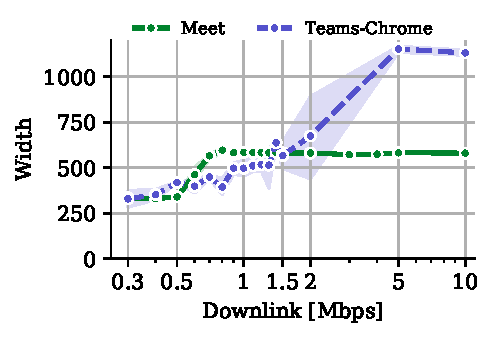
\includegraphics[width=\textwidth]{figures/static/downlink_received_frameWidth.pdf}
        \vspace{-2em}
    \caption{Frame width}
    \label{subfig:downlink_frame_width}
    \end{subfigure}
    \newline
        \begin{subfigure}[t]{0.3\textwidth}      
    		\centering
        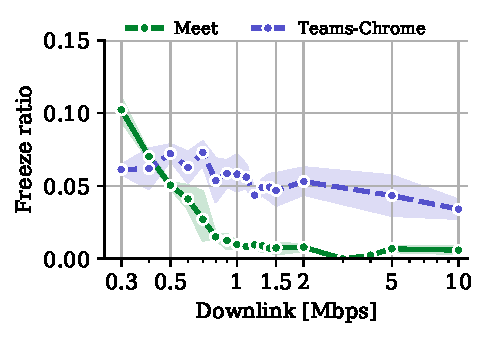
\includegraphics[width=\textwidth,keepaspectratio]{figures/static/downlink_freezeRatio.pdf}
        \vspace{-2em}
        \caption{Freeze ratio}
 		\label{subfig:downlink_freeze_ratio}
    \end{subfigure}%
    \hfill
	\begin{subfigure}[t]{0.3\textwidth}   
        \centering
        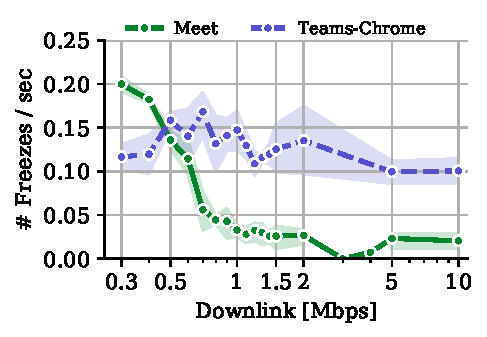
\includegraphics[width=\textwidth]{figures/static/downlink_freezeCountPerSecond.pdf}
        \vspace{-2em}
    \caption{Number of freezes per second}
    \label{subfig:downlink_freeze_per_sec}
    \end{subfigure}% 
    \hfill
	\begin{subfigure}[t]{0.3\textwidth}   
        \centering
        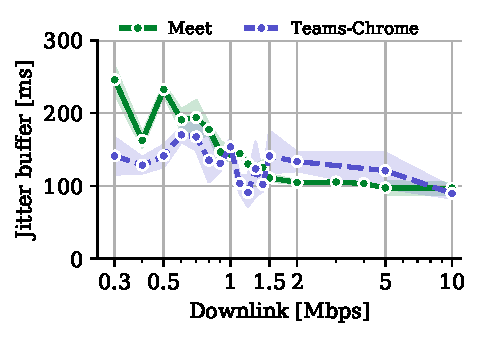
\includegraphics[width=\textwidth]{figures/static/downlink_jitter_buffer.pdf}
        \vspace{-2em}
    \caption{Jitter buffer delay}
    \label{subfig:downlink_jitter_buffer}
    \end{subfigure}
	\vspace{-1em}
	\caption{Downlink bandwidth and application performance metrics}
	\label{fig:downlink_application}
	%\vspace{-1em}
\end{figure*}



In this section, we study the impact of network capacity on the VCA performance. Each experiment consists of a 2.5-minute call between C1 and C2 under a specific shaping level. We conduct two set of experiments with downlink shaped in the first set and uplink shaped in the second set. We consider the following shaping levels: \{$0.3, 0.4, \dots, 1.5, 2, 5, 10$\} Mbps with 5 repetitions at each shaping level.  We also include the browser clients for \zoom and \teams, referred to as \zoombrowser and \teamsbrowser, respectively. This is done to understand if there are any platform-related differences. 
%% experiment setup
%% what is the experiment duration 
%% what bandwidth profiles are used 

% \tarun{Open questions: i) What about Team native client? ii) Audio performance? iii) Re-do \zoombrowser for 0.3 Mbps and 0.4 Mbps}



\subsection{Impact on network utilization} Figure~\ref{fig:downlink_bitrate} shows the median received network bitrate averaged over 5 runs for different downlink shaping levels. We find differences among VCAs in terms of their bitrate configuration and bitrate adaptation leading to different performance under same network conditions. For instance, the peak utilization for \teamsnative is $1.9$ Mbps whereas it is only $0.96$ for \zoomnative and $0.8$ Mbps for \meet. The received bitrate also reflects how different VCAs utilize the network especially under constrained links. Interestingly, we find that \zoomnative has the highest network utilization while \meet has the lowest (only $50\%$ at 0.5 Mbps) for downlink capacity lower than 0.75 Mbps. Finally, we also observe differences between \teamsbrowser and \teamsnative under same network conditions with the former having lower bitrates than the latter. For instance, at 1 Mbps shaping level, the received bitrate is only 0.5 Mbps for \teamsbrowser and 0.8 Mbps for \teamsnative. This suggests that implementation of the VCA can differ across platforms leading to different network and application behavior. 

\begin{figure}[t]
	%\vspace{-1em}
    \begin{subfigure}[t]{0.23\textwidth}      
    		\centering
        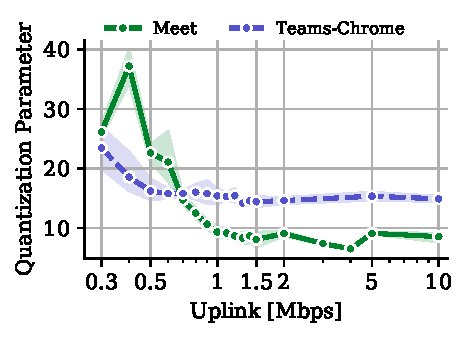
\includegraphics[width=\textwidth,keepaspectratio]{figures/static/uplink_s_qpsum.pdf}
        \vspace{-2em}
        \caption{Quantization parameter}
 		\label{subfig:uplink_video_quantization}
    \end{subfigure}%
\hfill
	\begin{subfigure}[t]{0.23\textwidth}   
        \centering
        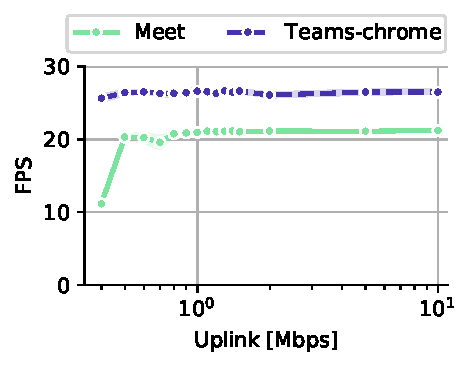
\includegraphics[width=\textwidth]{figures/static/uplink_sent_framesPerSecond.pdf}
        \vspace{-2em}
    \caption{Frames per second}
    \label{subfig:uplink_frames_per_second}
    \end{subfigure}% 
        \newline
    \hfill
	\begin{subfigure}[t]{0.23\textwidth}   
        \centering
        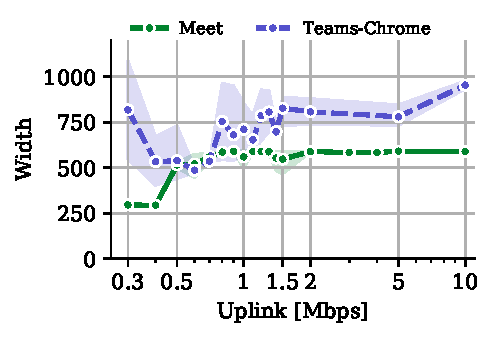
\includegraphics[width=\textwidth]{figures/static/uplink_sent_frameWidth.pdf}
        \vspace{-2em}
    \caption{Frame width}
    \label{subfig:uplink_frame_width}
    \end{subfigure}
        \begin{subfigure}[t]{0.23\textwidth}      
    		\centering
        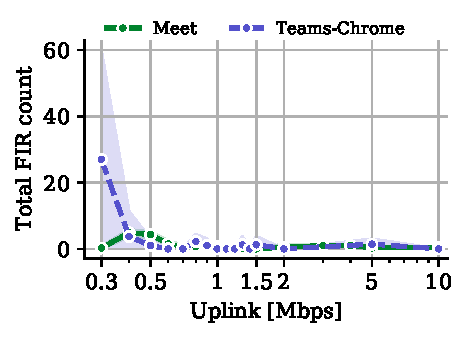
\includegraphics[width=\textwidth,keepaspectratio]{figures/static/uplink_sent_firCount.pdf}
        \vspace{-2em}
        \caption{FIR Count}
 		\label{subfig:uplink_fir}
    \end{subfigure}%
	\vspace{-1em}
	\caption{Uplink bandwidth and application performance metrics}
	\label{fig:uplink_application}
	%\vspace{-1em}
\end{figure}


\begin{table}[]
\centering
\begin{tabular}{|c|c|c|}
\hline
\textbf{VCA} & \textbf{\begin{tabular}[c]{@{}c@{}}Nominal bitrate \\ (Mbps)\end{tabular}} & \textbf{\begin{tabular}[c]{@{}c@{}}Observed \\ resolutions\end{tabular}} \\ \hline
\hline 
Meet         & 0.8                                                                        & x                                                                        \\ \hline
Teams        & 1.96 Mbps                                                                  & x                                                                        \\ \hline
Zoom         & 0.95 Mbps                                                                  & x                                                                        \\ \hline
\end{tabular}
\caption{Bitrate and resolutions for the VCAs}
\label{tab:vca_static}
\end{table}

\begin{figure*}[h!]
\begin{subfigure}[t]{.5\textwidth}
    \centering
    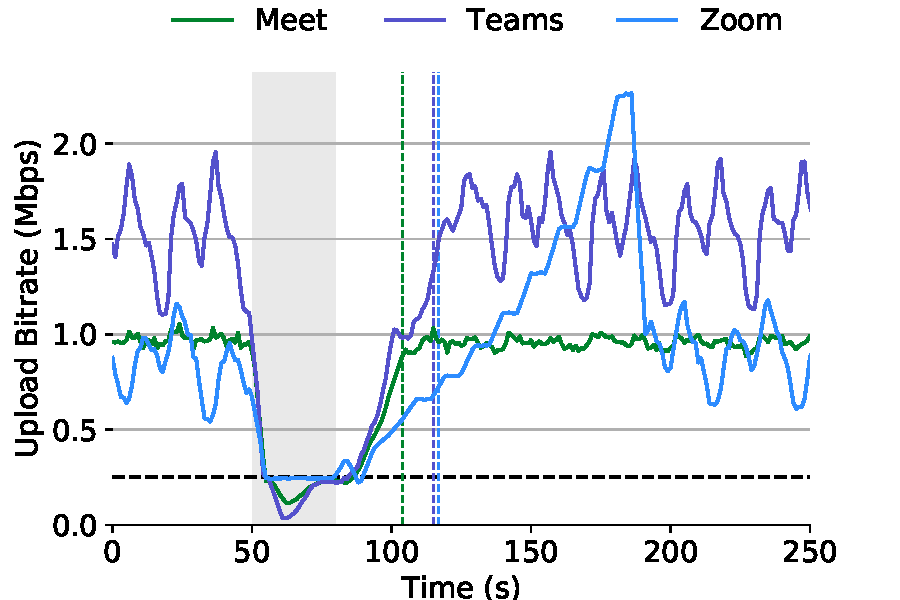
\includegraphics[width=\textwidth,keepaspectratio]{interrupt/Interrupt-upld.pdf}
    \captionsetup{width=.9\linewidth}
    \caption{Average uplink bitrate over time. Grey region indicates period where uplink capacity is constrained to 0.25 Mbps. Vertical dotted lines indicate when the uplink bitrate has returned to the average. Dotted horizontal line indicates the uplink shaping level.}
    \label{fig:ts_upld}
\end{subfigure}\hfill
\begin{subfigure}[t]{.5\textwidth}
      \centering
    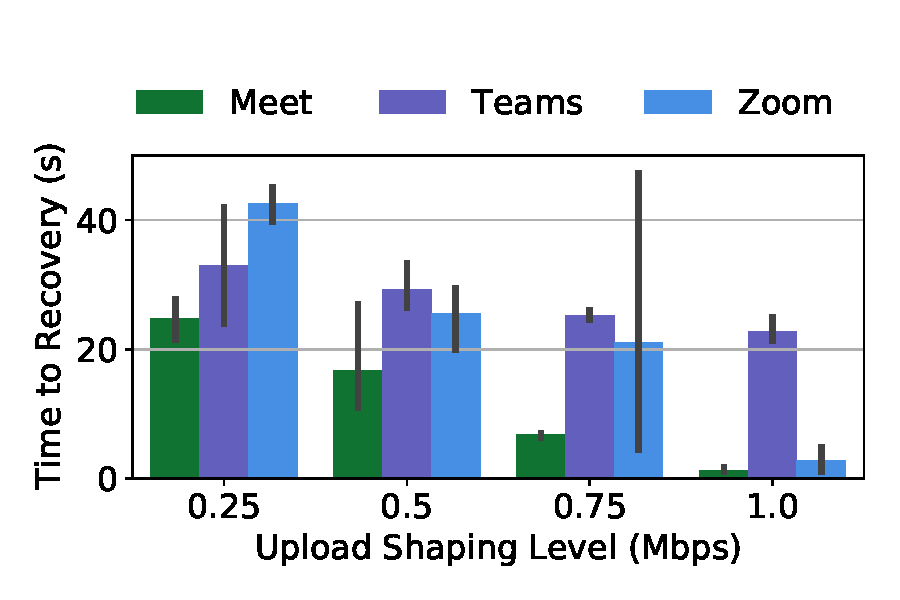
\includegraphics[width=1\textwidth,keepaspectratio]{interrupt/TTR-upld.pdf}
    \captionsetup{width=.9\linewidth}
    \caption{The time to recover to average sending bitrate following a drop to the indicated uplink shaping level}
    \label{fig:TTR_upld}
\end{subfigure}
\caption{VCA response to a 30s drop in available uplink capacity}
\label{fig:interrupt-upld}
\end{figure*}


We next analyze the median sent network bitrate for different uplink capacity (see Figure~\ref{fig:uplink_bitrate}). As expected, we find similar differences in terms of the maximum bitrate among the VCAs and between browser and native clients for \teams as observed in the downlink shaping experiment. However, the network utilization is higher, especially for \meet, when the upstream link is constrained as compared to downlink. Thus, there seems to be a discrepancy in bitrate adaptation when the upstream is constrained. We explore this discrepancy in more detail in Section~\ref{sec:interruption}. 

\subsection{Impact on application performance}
Here we describe how the link shaping level impacts application performance metrics. However, obtaining application metrics can be challenging for VCAs. We rely on WebRTC stats available on Google Chrome to obtain statistics for \teamsbrowser and \meet. We could not obtain the same statistics for \zoombrowser as it used different transport channels to transmit media, i.e., datachannels instead of the RTP MediaStream~\cite{webrtc_stats} as it may provides more flexibility (e.g., flexible encoding standards) to \zoom. However, video quality statistics are not exposed anymore through the WebRTC stats API. %In addition, we also obtained access to Zoom API through our campus network operator. The Zoom API provides limited application performance (e.g., video resolution, FPS) at a per-minute granularity~\cite{zoom_qos_api}. 
Thus, we limit this analysis to only \meet and \teamsbrowser for this section. 

%More specifically, we consider the following application metrics: Frames per second, video resolution, freeze ratio. 





\textbf{Application metrics and bitrate adaptation}: VCAs can ideally adapt the video bitrate by adjusting one or more of the following three parameters: i) frames per second (\textit{FPS}), ii) \textit{quantization parameter} used in image compression, and  iii) \textit{video resolution} indicating the number of pixels in each dimension. We indicate resolution with one of the dimension, i.e., \textit{frame width} in our analysis. Figure~\ref{fig:downlink_application} shows the above parameters for \meet and \teamsbrowser under different downlink shaping levels. 




We find that \teamsbrowser simultaneously degrades all three parameters as the downlink becomes more constrained. There is also significant variance across multiple repetitions under the same network bandwidth as shown by the $90\%$ confidence interval bands in the plot. \meet, on the other hand, follows a more consistent trend. In the 0.7-1 Mbps region, the bitrate is controlled mostly by adapting the FPS while keeping the quantization parameter and frame width similar to the nominal levels. However, after 0.7 Mbps, both \textit{resolution} and \textit{quantization parameter} degrade whereas there is an increase in the FPS. Below 0.5 Mbps, the frame width and the FPS stabilize while the quantization parameter actually reduces. It is not clear as to why \meet chose to reduce the quantization parameter after 0.5 Mbps and increase the FPS after 0.8 Mbps. 

We also plot the statistics related to video freezes during the call as obtained from the WebRTC stats. A freeze is assumed to occur if the frame inter-arrival is either greater than 3 $\times$ average frame duration or $150 ms$ + average frame duration.  Figure~\ref{subfig:downlink_freeze_ratio} and~\ref{subfig:downlink_freeze_per_sec} show the freeze ratio and number of freezes per second for \meet and \teamsbrowser. We find that both freeze ratio and freezes per second increase as the downlink bandwidth degrades. For \meet, the degradation is more severe than \teamsbrowser with $10\%$ freeze ratio at 0.3 Mbps. 


% Figure~\ref{fig:down}



\textbf{Takeaway}: VCA performance under same network conditions varies among tested VCAs. Further, the minimum bandwidth requirements have implications for broadband policy. The FCC currently recommends a 25/3 Mbps minimum connection. Such a connection would not suffice for two separate video conferences. A household with a parent working and a child attending class remotely would saturate the uplink and lead to poor user experience. 
%% also plot differences in network utilization and the shaping. 



%% Difference among VCAs. Peak utlization differs. For the same network conditions, VCAs peform differently. For instance, Teams on WebRTC 
%% Difference between native and browser client 
%% Google Meet Simulcast





\begin{comment}
\begin{figure}[t]
    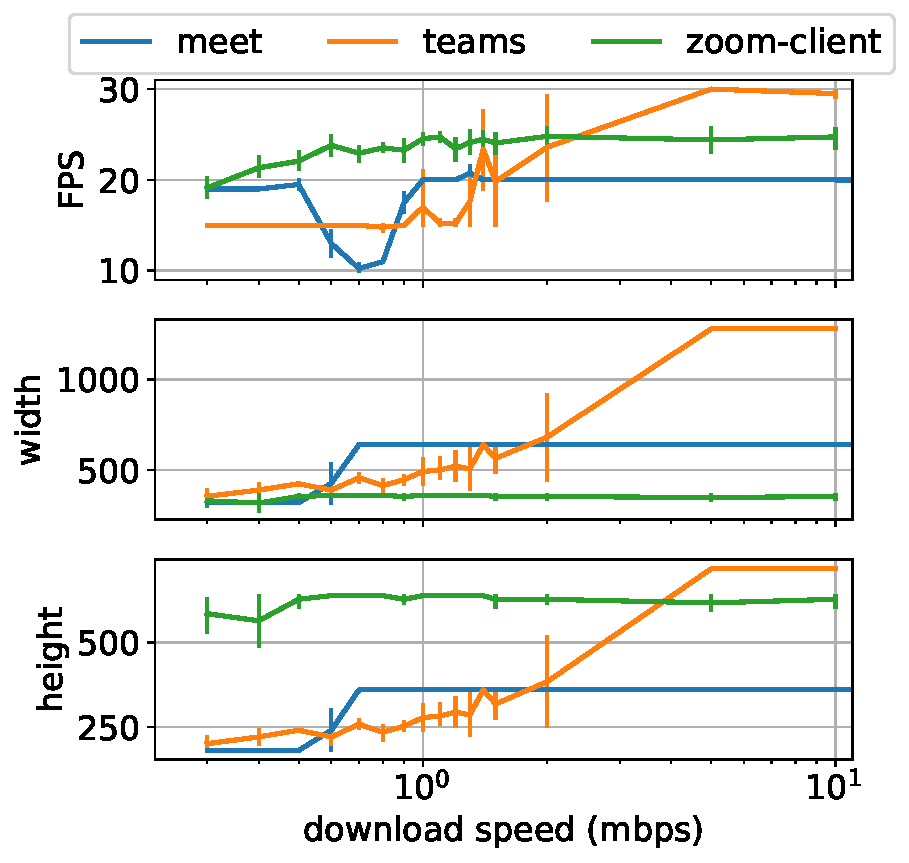
\includegraphics[width=0.35\textwidth,keepaspectratio]{figures/static/downlink_video_qual_meet_teams_zoom.pdf}
    \caption{Downlink bandwidth vs video quality \jamie{I think that width and height are almost always exactly redundant information.  I would choose one.  We should also keep the same colors across plots -- blue shouldn't be both Meet and Zoom client, for instance.}}
    \label{fig:downlink_video_qual}
\end{figure}


\begin{figure}[t]
    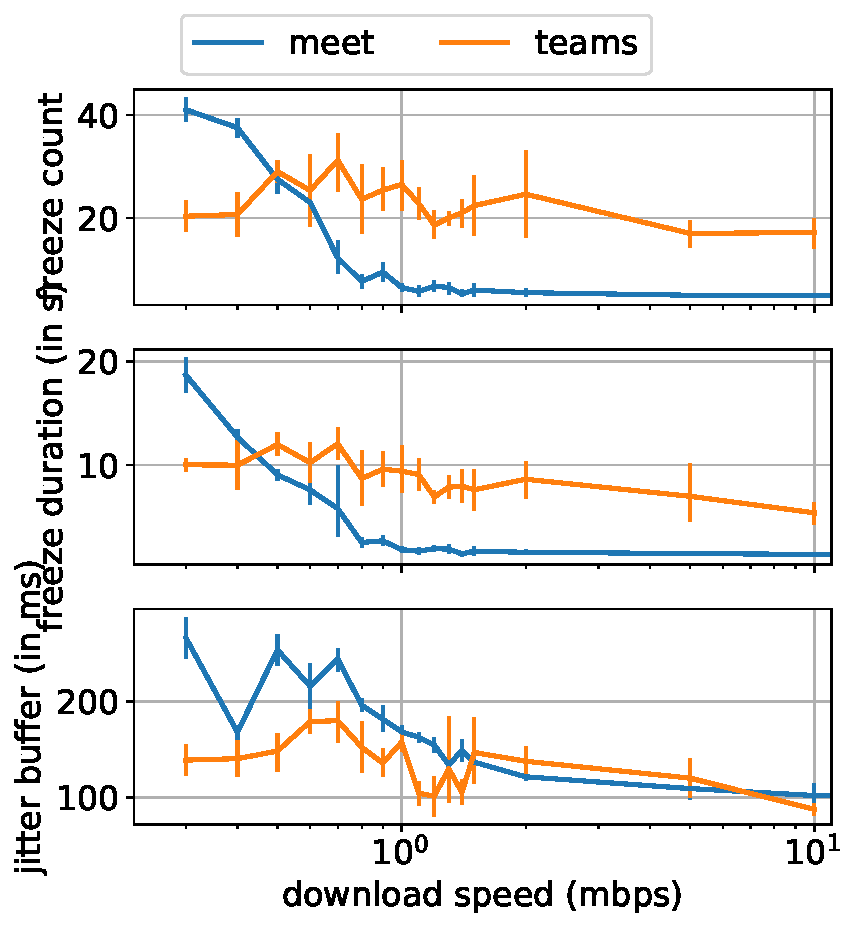
\includegraphics[width=0.35\textwidth,keepaspectratio]{figures/static/downlink_freeze_meet_teams.pdf}
    \caption{Downlink bandwidth and video freezes}
    \label{fig:downlink_freeze}
\end{figure}



\begin{figure}[t]
    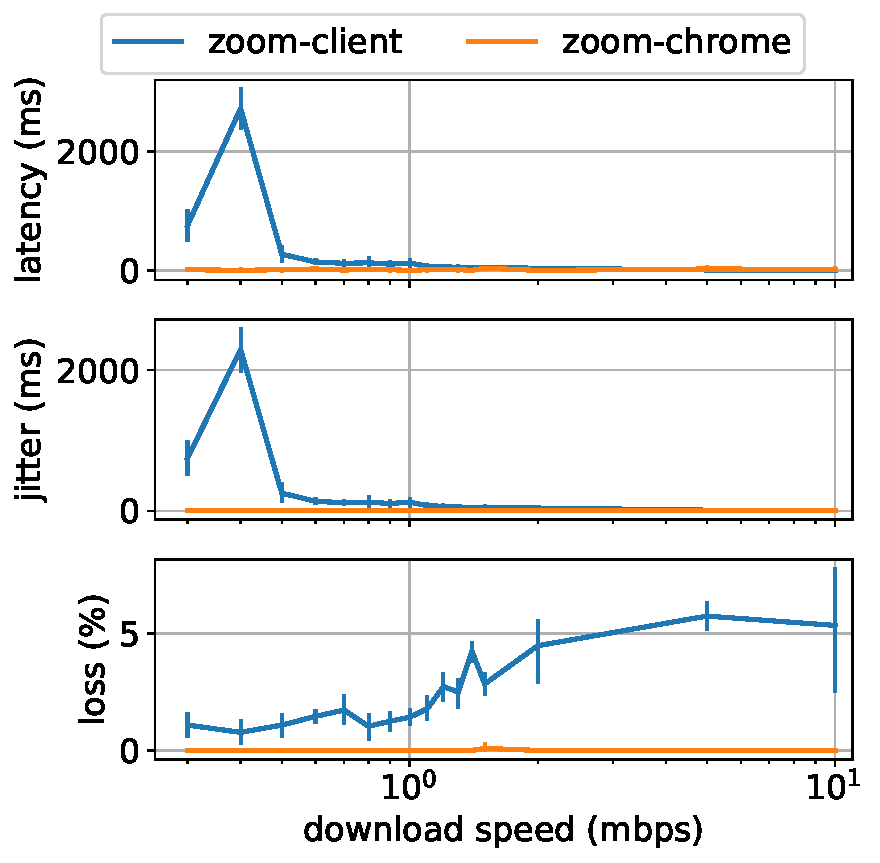
\includegraphics[width=0.35\textwidth,keepaspectratio]{figures/static/downlink_qos_zoom.pdf}
    \caption{Downlink bandwidth vs Zoom QoS. \jamie{It looks fishy, that zoom client latency and jitter are identical.  All data from browser seems to be zeroed out?}} 
    \label{fig:downlink_qos_zoom}
\end{figure}
\end{comment}


\section{Network Disruptions}
\label{sec:interruption}
One challenge in VCA design is deciding how to handle network disruptions. This challenge is especially pertinent as many use VCAs on home networks. Home networks are especially susceptible to disruptions caused by temporary congestion along the end-to-end path.

In this section, we analyze how VCAs respond to temporary network disruptions during the call by introducing transient drops in available bandwidth. Using the same setup as Figure \ref{fig:static_setup}, a 5-minute VCA call is initiated between two clients, C1 and C2, both of which sit behind unconstrained links. One minute after initiating the call, we reduce the available bandwidth between C1 and the router for 30 seconds, before reverting back to an unconstrained link. We conduct two sets of experiments, shaping the uplink in the first and the downlink in the second. We consider the following shaping levels: {0.25, 0.5, 0.75, 1.0} Mbps. We don't shape beyond 1.0 Mbps because both Zoom and Meet's average utilization is below 1.0 Mbps.

\begin{figure}[t!]
\centering
\begin{subfigure}[t]{.5\textwidth}
    \centering
    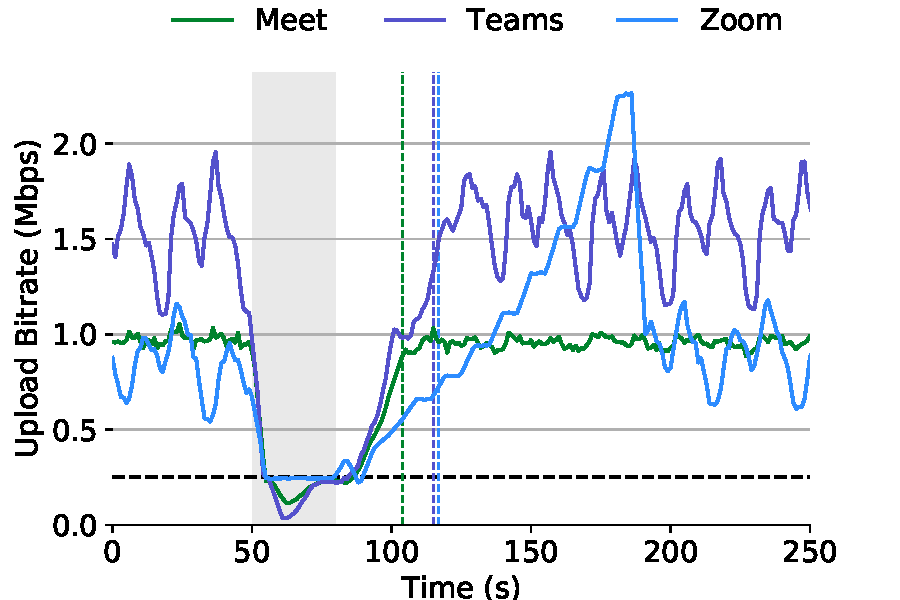
\includegraphics[width=.8\textwidth,keepaspectratio]{interrupt/Interrupt-upld.pdf}
    \caption{Average uplink bitrate over time. Grey region indicates period where uplink capacity is constrained to 0.25 Mbps. Vertical dotted lines indicate when the uplink bitrate has returned to the average.}
    \label{fig:ts_upld}
\end{subfigure}\hfill
\begin{subfigure}[t]{.5\textwidth}
      \centering
    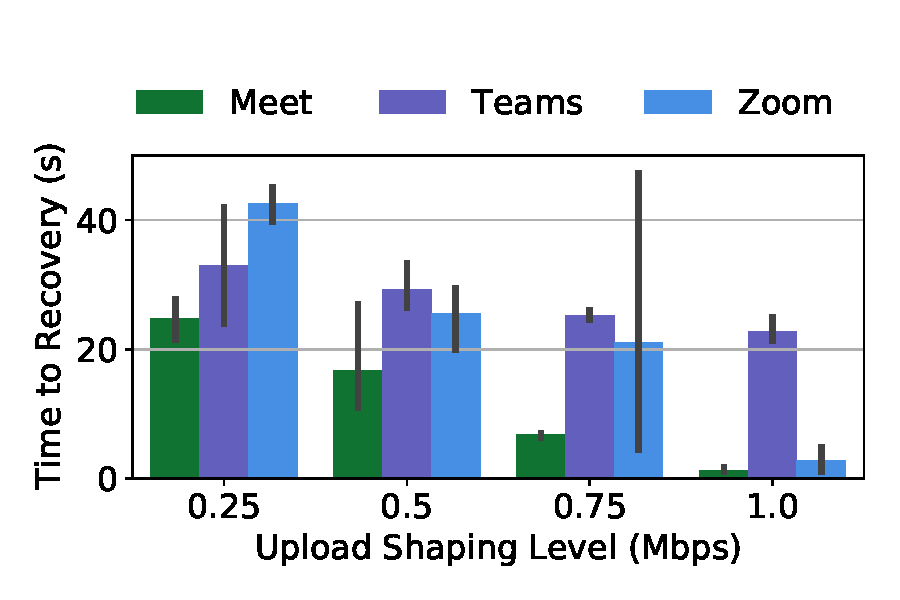
\includegraphics[width=.8\textwidth,keepaspectratio]{interrupt/TTR-upld.pdf}
    \caption{The time to recover to average sending bitrate following a drop to the indicated uplink shaping level.}
    \label{fig:TTR_upld}
\end{subfigure}
\caption{VCA response to a 30s drop in available uplink capacity}
\label{fig:interrupt-upld}
\end{figure}

\subsection{Uplink Disruptions}
Focusing first on uplink shaping, Figure \ref{fig:ts_upld} illustrates VCA uplink bitrate over the course of a call. It is clear that both the path to recovery and the time to recovery following an interruption differ greatly among the VCAs. We quantify the time it takes to VCA utilization to return to normal by introducing a metric called \textit{time to recovery} (TTR). We define TTR as the time between when the interruption ends and when the 5-second rolling median bitrate reaches the median bitrate before interruption, also referred to as nominal bitrate. %In other words, how long it takes the VCA performance to return to normal following the interruption. 

\paragraph{Time to Recovery}: Figure \ref{fig:TTR_upld} shows how the uplink shaping level affects each VCA's time to recovery. There is a clear trend that the more severe the uplink shaping, the longer the VCAs need to recover. This trend, however, is less pronounced for Teams than it is for Meet and Zoom as it takes longer to recover even at less severe shaping levels. This is because of two reasons: i) the nominal bitrate of Teams is higher than Meet and Teams, ii)  Teams increases the uplink bitrate slowly immediately after the interruption before increasing quickly back to normal (see  Figure~\ref{fig:ts_upld}), almost resembling a cubic function. Meet also observes this cubic-like recovery at the 0.25 Mbps shaping level. However, it recovers much faster at other shaping levels, mostly because its nominal bitrate is around 0.96 Mbps. 

\paragraph{Recovery Patterns}: While Meet and Teams seem to follow a cubic-like trendline, Zoom's recovery is markedly different. It takes the longest time to recover under severe interruptions. Looking at Figure \ref{fig:ts_upld}, Zoom follows a stepwise recovery, with an almost-linear increase right after interruption. It then enters into a periodic-probing phase where it increases the sending rate, stays at it for sometime before increasing it again. The probing phase continues well above the its nominal bitrate, before finally dropping back. Zoom does not return to a ``normal'' sending pattern until 2 minutes after the interruption, sending at much higher rates than necessary. At first look, such probing seems like a bad design as it introduces packet loss on the link, hurting Zoom's own performance let alone others. However, we believe that Zoom may be using redundant FEC packets to gauge available bandwidth similar to the FBRA congestion control proposed by Nagy et al.~\cite{nagy2014congestion}. Thus, even if there is packet loss, the user performance does not suffer. This inefficient use of the uplink, however, could disturb other applications on the same link, leading to a poor quality of experience for competing applications. 

\begin{figure}[t!]
 \centering
\begin{subfigure}[t]{.5\textwidth}
   \centering
    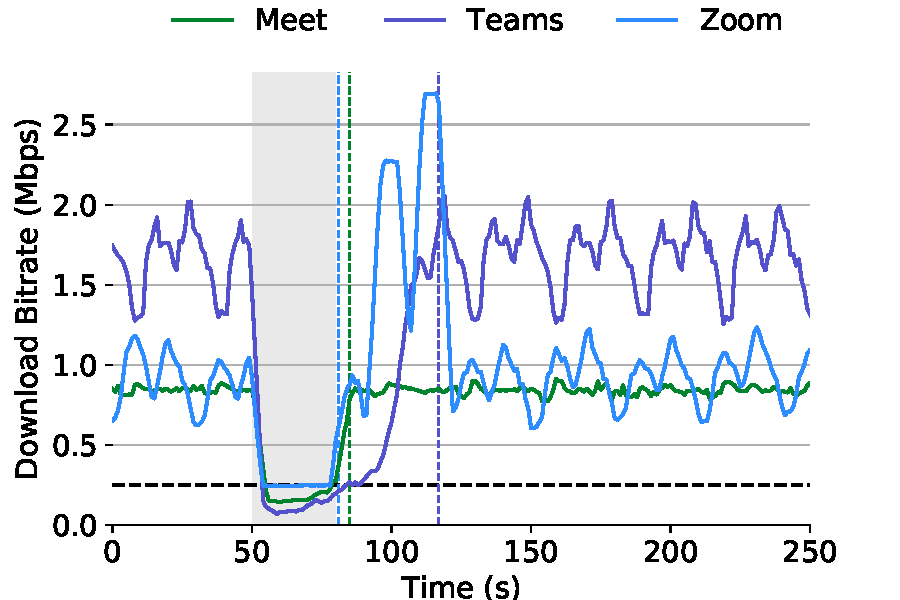
\includegraphics[width=.9\textwidth,keepaspectratio]{interrupt/Interrupt-dnld.pdf}
    \caption{Average downlink bitrate over time. Grey region indicates period where downlink capacity is constrained to 0.25 Mbps. Vertical dotted lines indicate when the dowlink bitrate has returned to the average.}
    \label{fig:ts-dnld}
\end{subfigure}
\begin{subfigure}[t]{.5\textwidth}
  \centering
    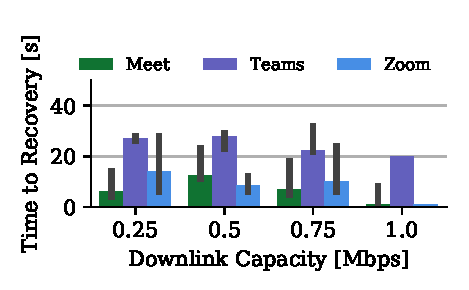
\includegraphics[width=.9\textwidth,keepaspectratio]{figures/interrupt/TTR-dnld.pdf}
    \caption{The time to recover to average receiving bitrate following a drop to the indicated downlink shaping level.}
    \label{fig:TTR_dnld}
\end{subfigure}
\caption{VCA response to a 30s drop in available downlink capacity.}
\label{fig:interrupt-dnld}
\end{figure}

\subsection{Downlink Disruptions}

Turning now to downlink shaping, it is clear from Figure~\ref{fig:TTR_dnld} that Teams recovers much slower than Meet and Zoom, always taking at least 20 seconds longer to return to the average rate, regardless of the magnitude of the interruption. Furthermore, Meet and Zoom recover much faster in this case compared to uplink interruptions. This can be explained by the way each VCA sends video. In all three VCAs, C1 and C2 communicate through an intermediary server. Thus, the recovery times depend on the congestion control capabilities at the server. 


As mentioned in Section~\ref{sec:static}, Meet uses an encoding technique called \textit{simulcast}, where the client encodes two versions. The server then sends the appropriate version based on the perceived downlink capacity at the receiver. This way, a sender transmitting on an unconstrained link does not have to adjust its sending and can rely on the server to send the appropriate version. The server can then quickly switch between which version to send to the receiver based on the feedback it receives. This quick recovery is clearly illustrated in \ref{fig:interrupt-dnld}, in which Meet returns to its average rate in under 10 seconds, regardless the severity of the interruption.

Similarly, Zoom uses \textit{scalable video coding} when transmitting video~\cite{zoom_encoding}. Instead of sending several versions of varying quality, Zoom sends many hierarchical "layers" that, when superimposed, produce a high quality video. This allows C2 to continue sending uninterrupted even when C1's downlink capacity shrinks. The server can then recover faster by sending additional layers, once the network conditions improve.  


\begin{figure}[t]
    \centering
    \includegraphics[width=0.45\textwidth,keepaspectratio]{../figures/interrupt/Interrupt-sender.pdf}
    \caption{Client 2 (C2) uplink bitrate. Grey region indicates when C1's downlink capacity is reduced to 0.25 Mbps}
    \label{fig:interrupt-sender}
\end{figure}

\begin{figure}[]
   \centering
    \includegraphics[width=0.5\textwidth,keepaspectratio]{methodology/competition-setup.pdf}
    \caption{Setup for competition experiments.}
    \label{fig:competition-setup}
\end{figure}

\begin{comment}
 \begin{figure*}[t]
    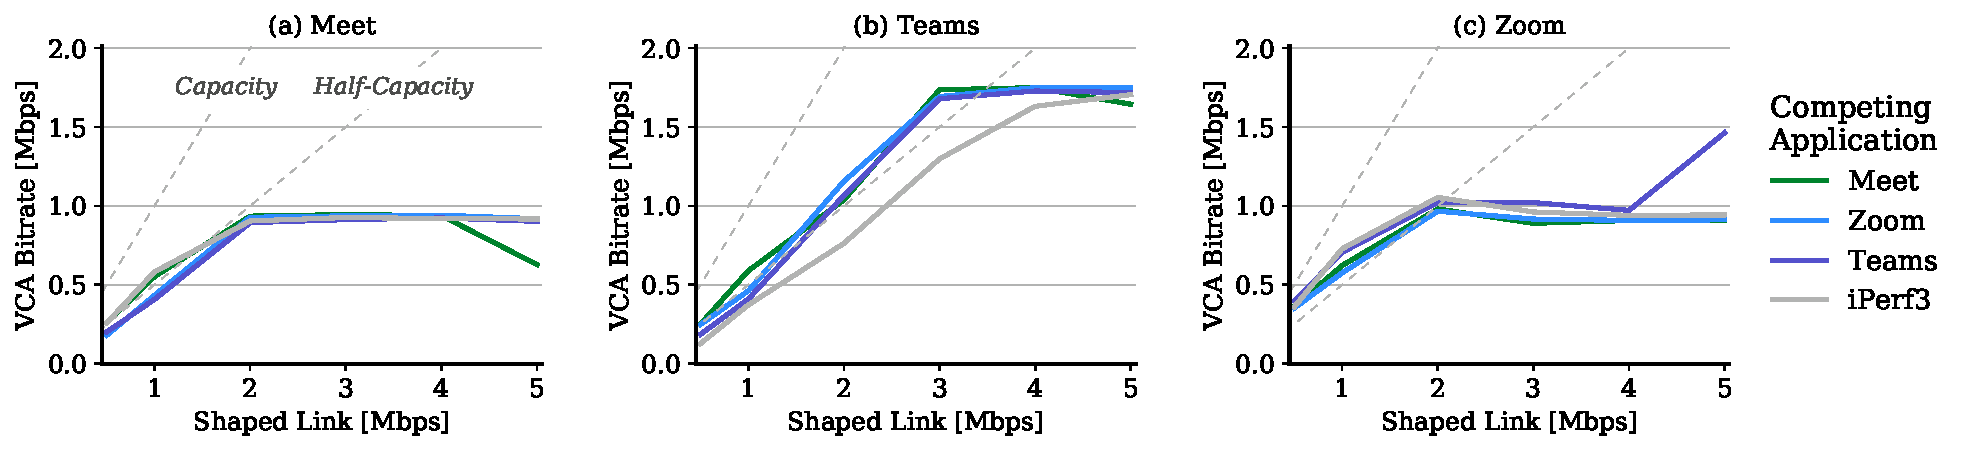
\includegraphics[width=\linewidth]{comp/ul_competition_all.pdf}
    \caption{Share of upstream link and VCA bitrates for VCAs in competition with other flows, as a function of downlink bitrate cap.}
	\label{fig:comp_bitrates_ul}
\end{figure*}
\end{comment}


\begin{figure*}[t!]
    \centering
    \begin{subfigure}[t]{.33\textwidth}
        \centering
        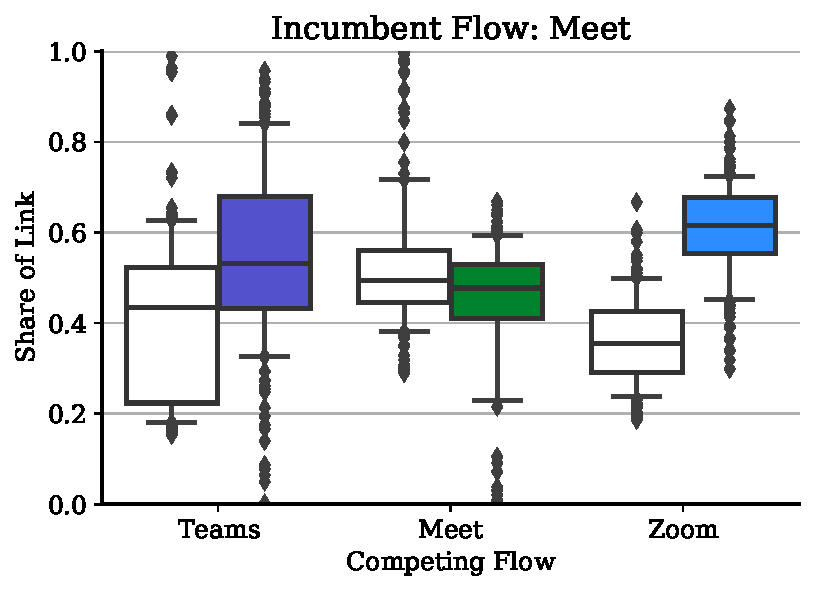
\includegraphics[width=1\textwidth]{figures/comp_all/box_plot_meet_ul_0.5_all.pdf}
        \caption{Meet}
        \label{fig:meet_ul_box}
    \end{subfigure}\hfill
    \begin{subfigure}[t]{.33\textwidth}
        \centering
        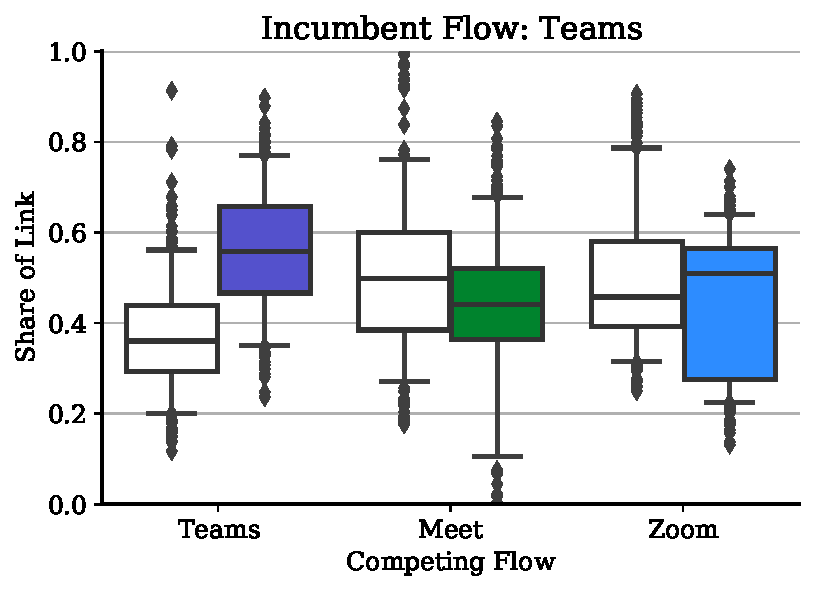
\includegraphics[width=1\textwidth]{figures/comp_all/box_plot_teams_ul_0.5_all.pdf}
        \caption{Teams}
        \label{fig:teams_ul_box}
    \end{subfigure}
    \begin{subfigure}[t]{.33\textwidth}
        \centering
        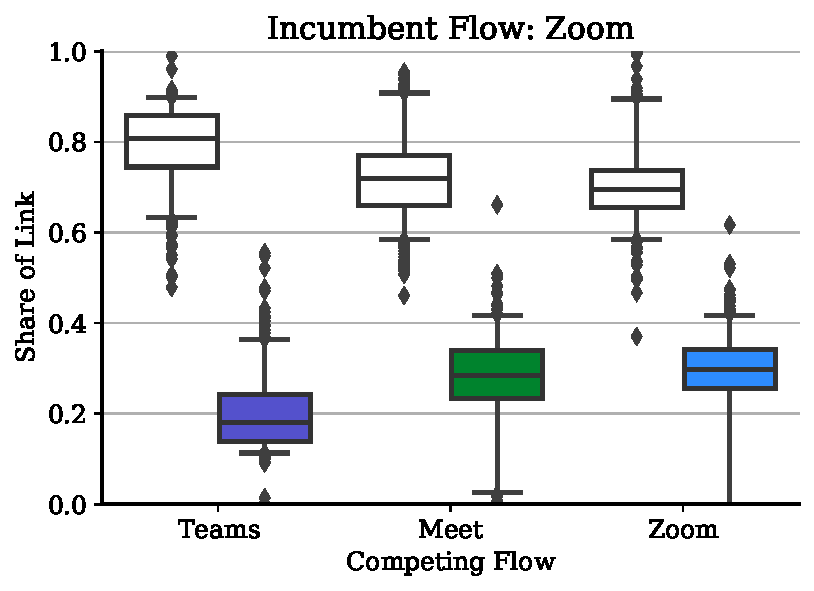
\includegraphics[width=1\textwidth]{figures/comp_all/box_plot_zoom_ul_0.5_all.pdf}
        \caption{Zoom}
        \label{fig:zoom_ul_box}
    \end{subfigure}
    \caption{Uplink bitrate of applications in competition with each VCA, with a link shaped symmetrically at 0.5~Mbps.}
    \label{fig:boxplot-upld}
\end{figure*}




While the intermediary server for Zoom and Meet does congestion control, it only acts as a relay for Teams. During a Teams call, C2 will recognize C1 has limited downlink capacity and adjust its behavior, sending at only the bitrate it knows C1 can handle. Once C1 has more available bandwidth, however, C2 must first probe the connection before returning to its average sending rate. Figure \ref{fig:interrupt-sender} illustrates how C2's sending rate does not change during a Meet call, but drops below the shaping threshold during a Teams call, leading to the slow recovery.


In terms of how efficiently each VCA uses the constrained link, Zoom's downlink and uplink bitrate stays at the shaping level while Meet and Teams fall even lower than the shaping level. Zoom's efficient network utilization may be an artifact of its encoding mechanisms, wherein it can more effectively control the encoding parameters (e.g., svc-encoded layers, FPS, resolution etc.) to match the target bitrate.  

\begin{mdframed}[roundcorner=5pt, backgroundcolor=black!10]
\noindent \textbf{Takeaways}: VCAs are slow to recover from reduction to uplink capacity, all requiring over 25 seconds to recover from severe interruptions to 0.25 Mbps. Only Teams is consistently slow to recover from drops in downlink capacity, even following moderate drops to 1 Mbps. This result can be attributed to VCA's media sending mechanism and how  congestion control is implemented at the intermediate server for each VCA. 
\end{mdframed}



\begin{figure}[]
   \centering
    \includegraphics[width=0.5\textwidth,keepaspectratio]{../figures/methodology/competition-setup.pdf}
    \caption{Setup for competition experiments}
    \label{fig:loss_latency}
\end{figure}

\section{Competing Flows}
To test how VCAs handle fairness on a constrained link, we launch a competing application on the same network. We define three sets of competing applications: VCAs, video streaming, and file transfer. We use Meet, Teams, and Zoom for the VCAs, Youtube and Netflix for video streaming, and iPerf3 TCP for file transfer. The competing VCAs are initiated as described above. We play the same gaming video and the same movie on Youtube and Netflix, respectively, for every experiment using \texttt{xdg-open}. Finally, iPerf3 is started as usual on the command line.
Two fundamental questions:
\begin{enumerate}
    \item are the apps fair WRT each other, WRT traditional flows (TCP), and other applications (YouTube, NetFlix)
    \item for two flows, what link capacity is required for full performance?
\end{enumerate}

\jamie{part of what feels weird to me, in using download flows, is that these are SO MUCH lower than what most people by, that they feel irrelevant.  If we had upstream, these same numbers would not be unreasonable, for the ``popular discourse" on broadband thresholds.}

\noindent \textbf{Methodology}.



The experiment is built within the framework already described.
The distinguishing feature of this measurement is that the 
  constrained link is between a switch and an OpenWRT Router 
    (which constrains the link).
The router has a gigabit link to the Internet.
The competing flows are initiated from two matched consumer laptops,
  connected to the switch over unconstrained, gigabit links.
We consider three forms of competitive flows:
  a standard TCP flow through iperf3 with cubic congestion control,
  other video conferencing applications, and 
  common video streaming services.
The ``counter-parties" for these flows are, respectively,
  a dedicated server on the university network,
  consumer laptops, and industry servers.
In contrast to previous experiments, 
  we focus on the native versions of Zoom and Teams clients.
\jamie{Awkward: Meet is native in Chrome.}

Each single experiment lasts for 4 minutes.
The ``nominal flow" is established first, and
  and the competing flow follow 30 seconds later.
The competing flow lasts for 2.5 minutes.
The experiment concludes with 1 minute
  with the nominal flow alone.
This setup is illustrated in Figure~\ref{fig:ts_zoom_netflix},
  with the time series for a six experiments between Zoom and Netflix.
Each configuration of nominal and competing flows and link constraint
  is repeated five times.
The capacity constraints are to 0.5, 1, 2, 3, 4, and 5 Mbps.
Bitrates are measured from packet captures.
  
\begin{figure}[]
    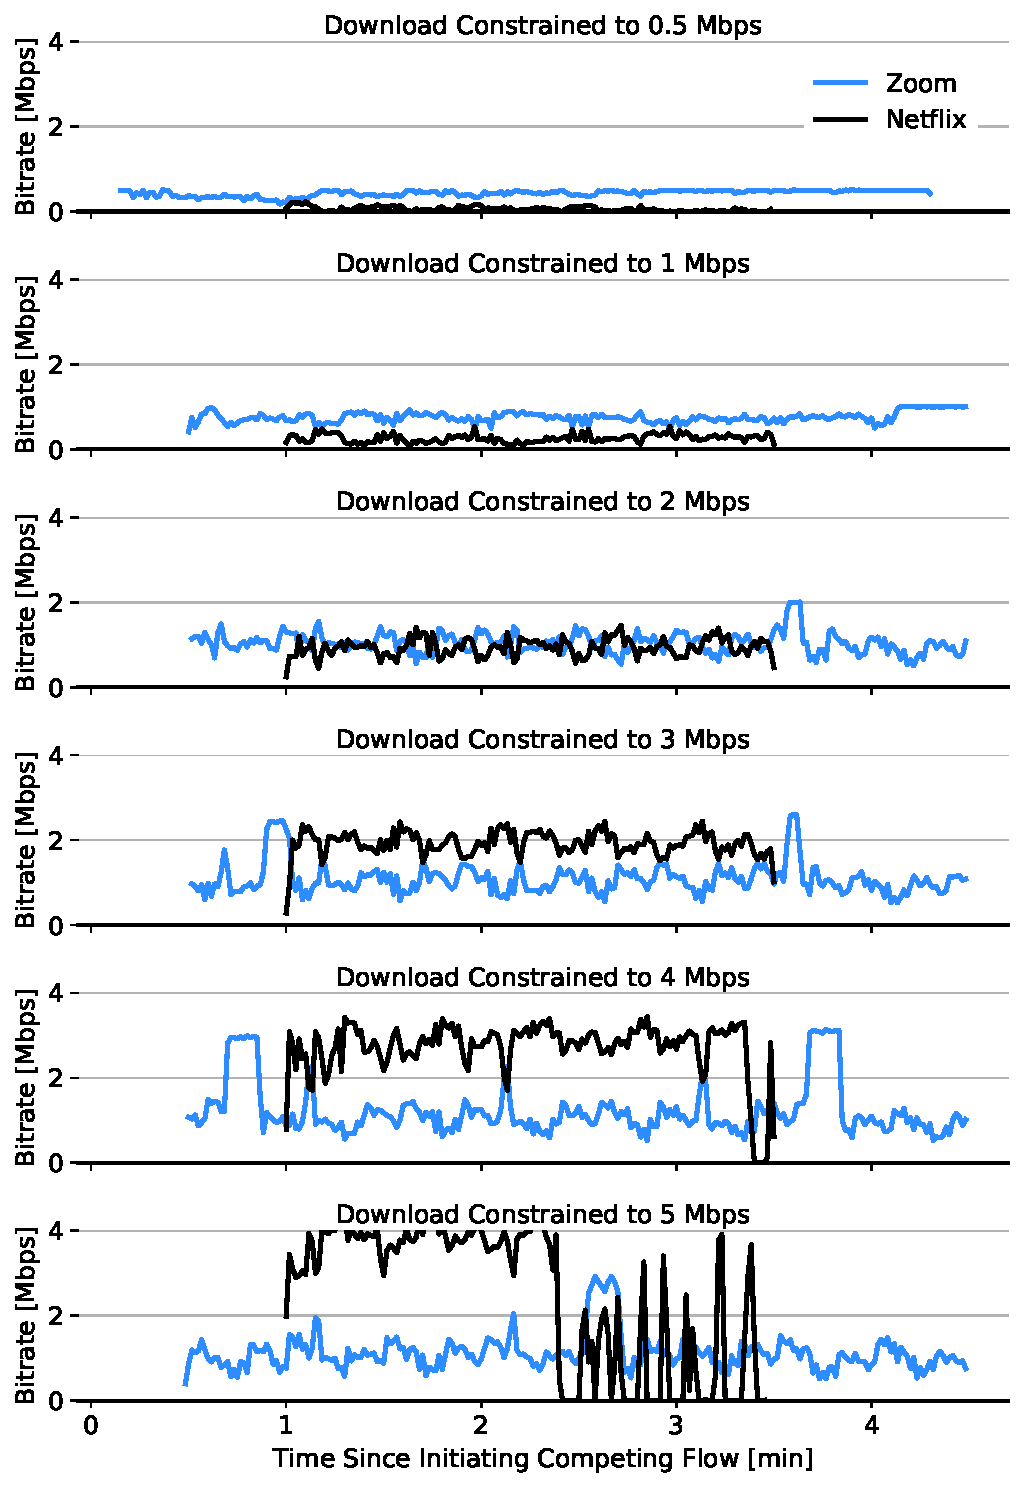
\includegraphics[width=\linewidth]{comp/zoom_netflix_dl_time_series.pdf}
    \caption{Time series of bitrate for Zoom in competition with a Netflix flow, at different link capacity. \jamie{timing offset bug}}
	\label{fig:ts_zoom_netflix}
\end{figure}

\begin{figure}[]
    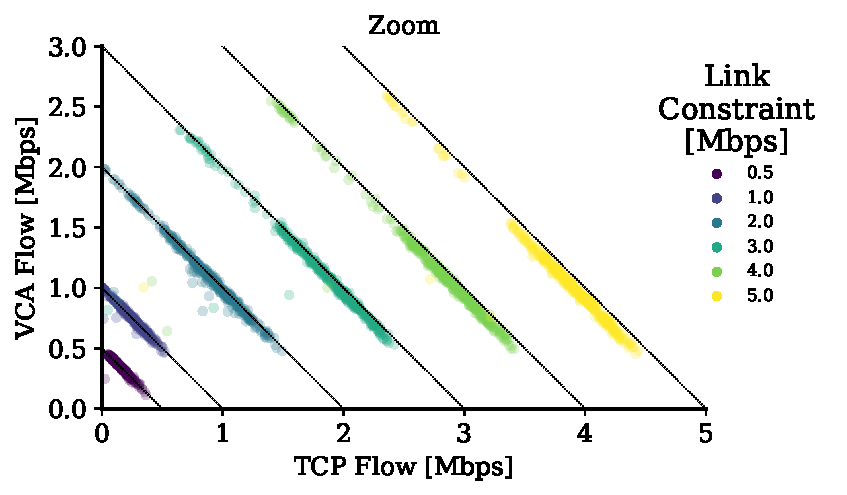
\includegraphics[width=\linewidth]{comp/zoom_iperf_scatter.pdf}
    \caption{Competition between Zoom and an iperf3 TCP flow. \jamie{kind of pretty, but not obviously useful}}
	\label{fig:comp_zoom_iperf}
\end{figure}

\begin{figure}[]
    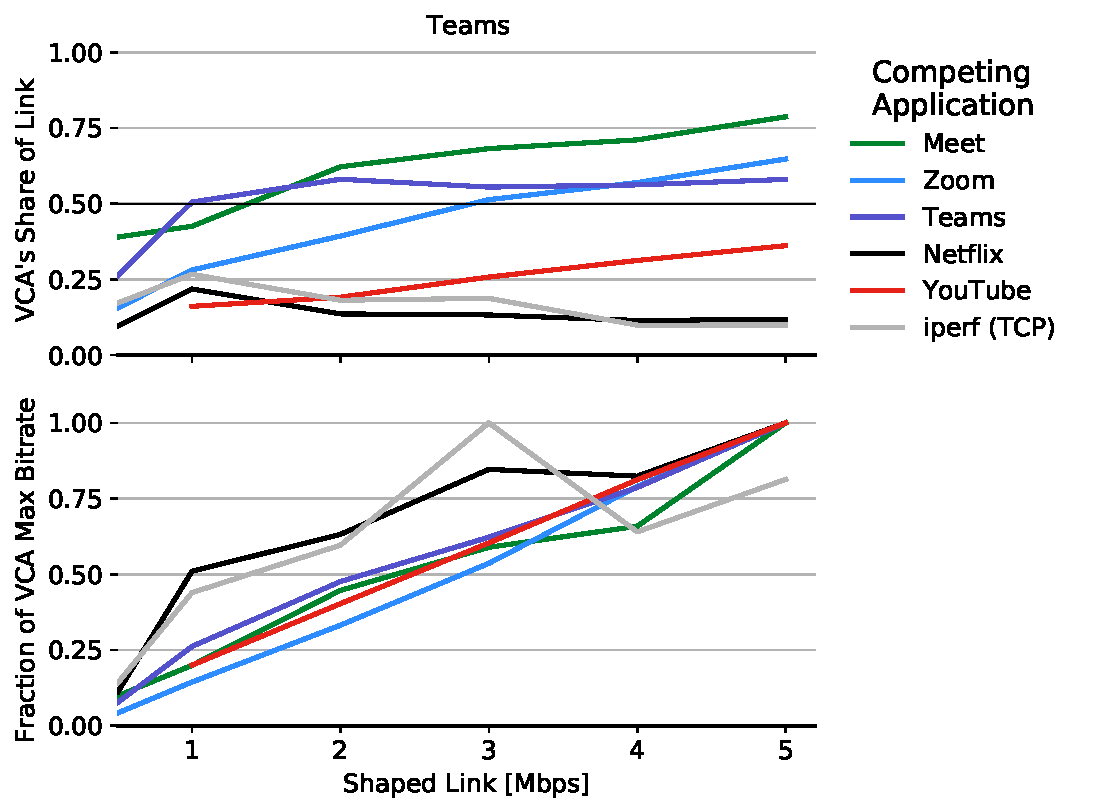
\includegraphics[width=\linewidth]{comp/teams_competition.pdf}
    \caption{Link share and share of nominal bitrate for Teams, in competition with other flows, as a function of downlink bitrate cap. \jamie{Combine this and following figures into one full-width / 6-panel figure.  Increase font sizes, etc.}}
	\label{fig:teams_comp_bitrates}
\end{figure}

\begin{figure}[]
    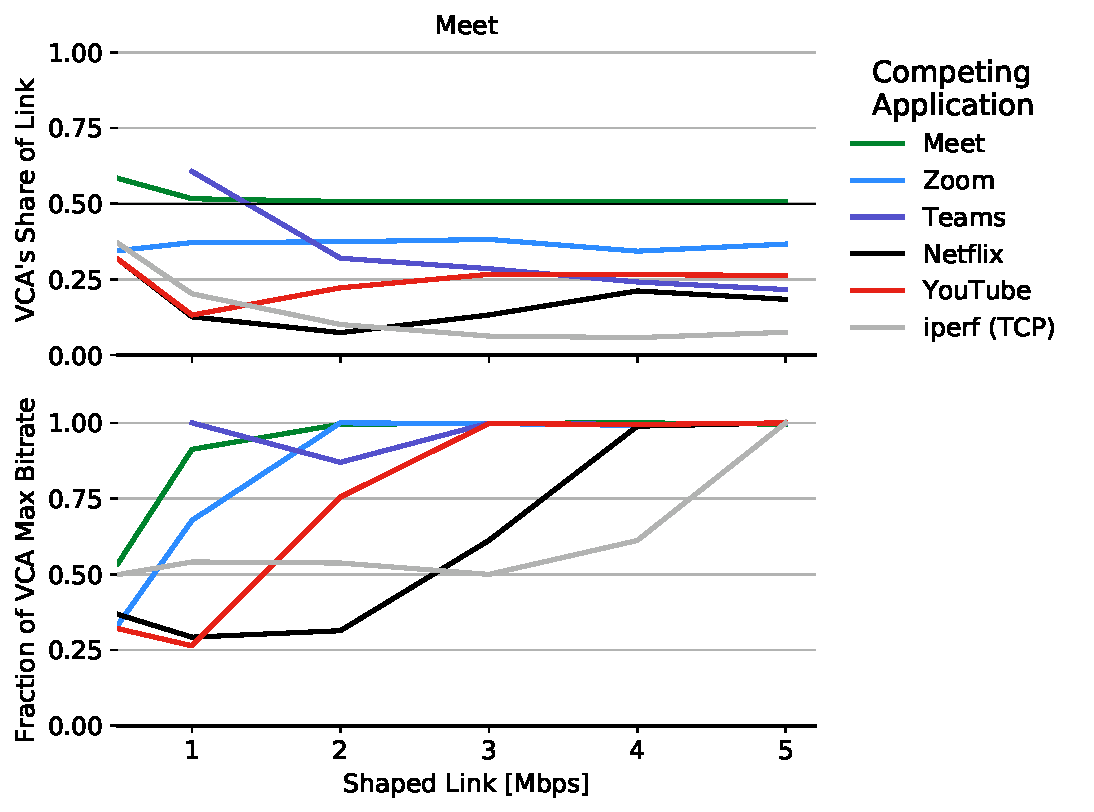
\includegraphics[width=\linewidth]{comp/meet_competition.pdf}
    \caption{Link share and share of nominal bitrate for Meet, in competition with other flows, as a function of downlink bitrate cap.}
	\label{fig:meet_comp_bitrates}
\end{figure}

\begin{figure}[]
    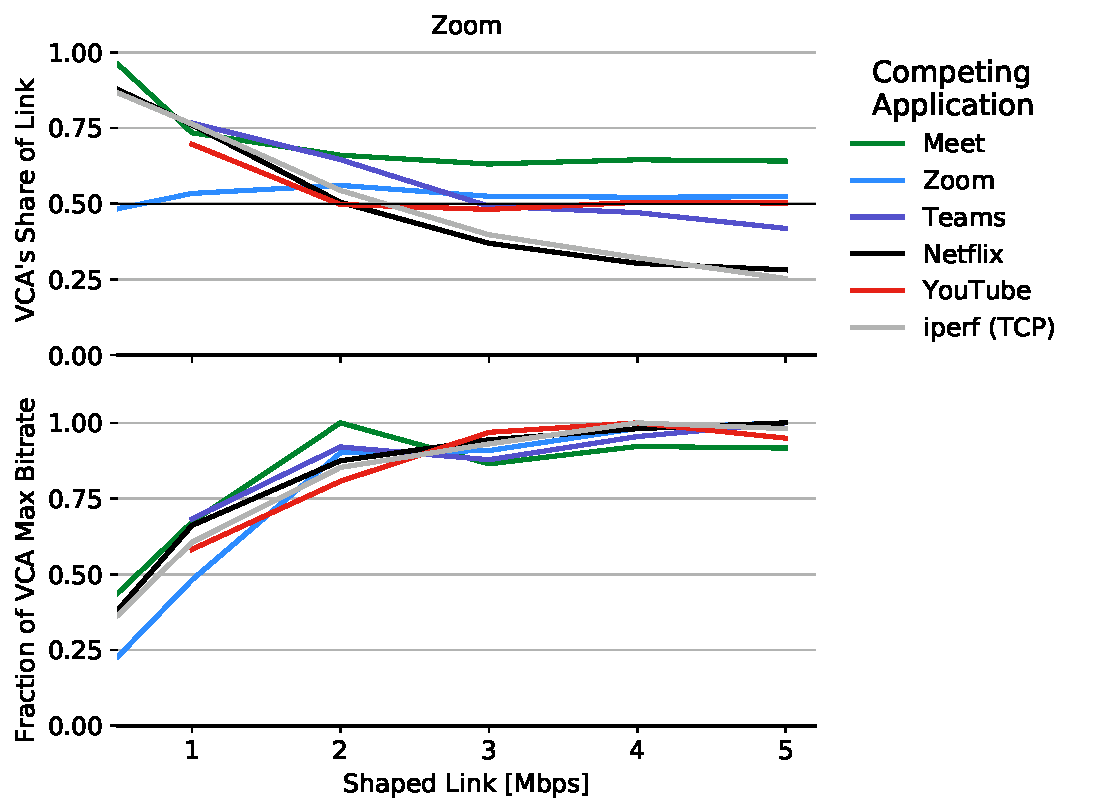
\includegraphics[width=\linewidth]{comp/zoom_competition.pdf}
    \caption{Link share and share of nominal bitrate for Zoom, in competition with other flows, as a function of downlink bitrate cap.}
	\label{fig:zoom_comp_bitrates}
\end{figure}

\begin{figure}[]
    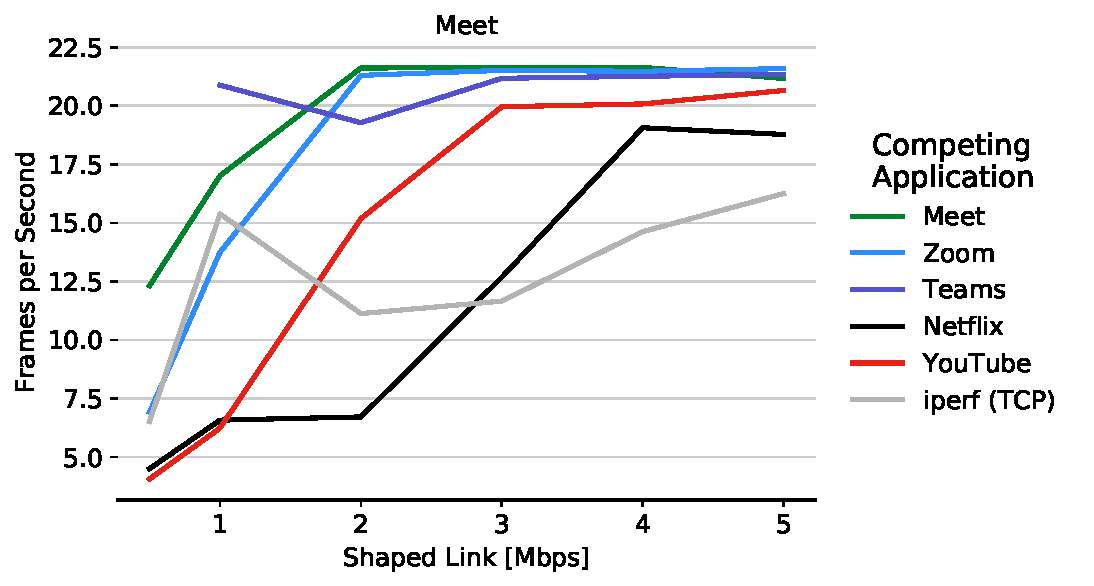
\includegraphics[width=\linewidth]{comp/meet_performance.pdf}
    \caption{Meet frames per second, in competition with other flows and as a function of link capacity.}
	\label{fig:meet_comp_performance}
\end{figure}



From these flows we construct two variables
  to reflect fairness and performance.
Fairness is represented 
  as the nominal flow's share of the constrained link.
Performance is the flow's share of its bitrate 
 as measured on a fully unconstrained call (see Table~\ref{}).
\jamie{The fully-unconstrained values are important benchmarks that we should measure carefully.  I know Tarun quoted these.  But we should establish these and put them in a table early on.}
Figures~\ref{fig:teams_comp_bitrates}-\ref{fig:zoom_comp_bitrates}
  display results for Teams, Meet, and Zoom respectively.

Each application in ``competition" with itself, uses half the link.
Competition is in evidence primarily at the low end of the domain,
  with the most severe constraints.
With weaker constraints, most applications reach their nominal bitrates
  and the ratios in the upper panels simply show the ratio of their bandwidth demands.
For example, 
  the low VCA shares with respect to iperf at weak constraint
  simply illustrates the "inexhaustible" demand of a TCP flow,
  whereas link share's of Zoom vs Meet or Meet vs Zoom 
  at link capacity of 5 Mbps (0.4 or 0.6) simply 
  reflect the nominal bandwidths.

\jamie{ambiguity: NetFlix or YouTube buffering, vs slow-start from teams}
  
At the low end, Zoom competes
  aggressively and effectively with all other flows:
  it consumes nearly the entire link against Meet (\textcolor{red}{95\%}), 
  and \textcolor{red}{80\%} of the link against Teams.
Both Teams and Meet fare worse on constrained links.
  
The lower panels of the figures show
  the link bandwidth required for the VCAs' consumption
  to converge to their nominal levels.
Again, Zoom is quick out of the gate, and 
  achieves over \textcolor{red}{90\%} of nominal link bitrate,
  for constraints weaker than 2 Mbps.
On the other hand, Teams does not achieve full bitrate
  until \jamie{we gotta run higher..}
Depending on the flow, Meet achieves full 
  performance when the shared link has capacity greater than 3 Mbps, 
  except for the (unlimited) TCP flow.
  
\jamie{Zoom competing with meet nominal is flat, whereas the inverse is not.  These aren't exactly the same -- there's an ``incumbency" advantage -- but worth noting.}

\jamie{Add notes on performance, e.g., through Meet, though I think that the preceding is most of the story.}


% \begin{figure}[]
%     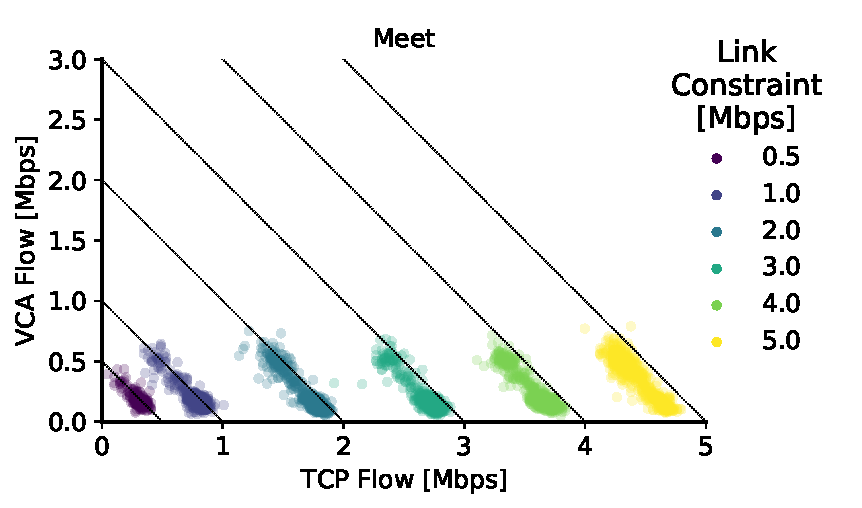
\includegraphics[width=\linewidth]{comp/meet_iperf_scatter.pdf}
%     \caption{Competition between Meet and an iperf3 TCP flow.}
% 	\label{fig:comp_meet_iperf}
% \end{figure}

% \begin{figure}[]
%     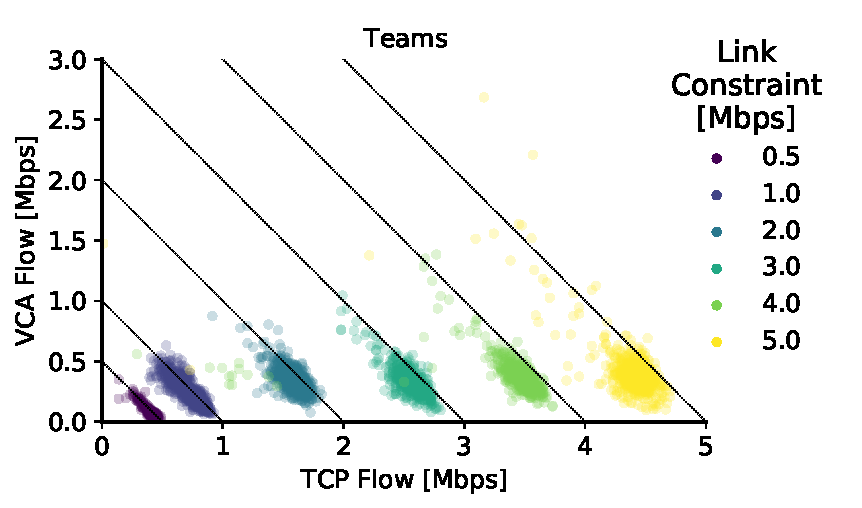
\includegraphics[width=\linewidth]{comp/teams_iperf_scatter.pdf}
%     \caption{Competition between Teams and an iperf3 TCP flow.}
% 	\label{fig:comp_teams_iperf}
% \end{figure}


\section{Application context and network consumption}\label{sec:usage_modality}
In this section, we analyze the impact of different usage modalities such as the number of persons in the call, viewing mode, and device type on the network consumption. 
\subsection{Number of Users}
\subsection{Viewing Mode}

\section{Related Work}\label{sec:related}

\textbf{VCA measurement}: Some of the early VCA measurement work has focused on uncovering the design of the Skype focusing on its streaming protocols~\cite{baset2004analysis}, architecture~\cite{guha2005experimental}, traffic characterization~\cite{bonfiglio2008tracking}, and application performance~\cite{hossfeld2008analysis}. More recent work has included other VCAs and streaming contexts~\cite{xu2012video, yu2014can, azfar2016android}. Xu et al.~\cite{xu2012video} use controlled experiments to study the design and performance of Google+, iChat, and Skype. The work is further extended to include performance of the three services on mobile video calls~\cite{yu2014can}. 

Closest to our work is work by Jansen et al.~\cite{jansen2018performance} and Nistico et. al~\cite{nistico2020comparative}. Jansen et al. evaluate WebRTC performance using their custom VCA under controlled network conditions~\cite{jansen2018performance}. Emulating similar network conditions, we consider performance of commercial and more recent VCAs that widely used for education and work. Even between tested VCAs using WebRTC, namely \meet and \teamsbrowser, we find significant performance differences, likely due to different design parameters (e.g., codecs, default bitrates). Nistico et al.~\cite{nistico2020comparative} consider a wider range of recent VCAs, focusing on their design differences including protocols and architecture. Our work provides a complimentary performance analysis for a subset of the VCAs studied by them. We use the insights from their work to explain the differences among VCAs' network utilization and performance under similar streaming contexts. 

\textbf{VCA congestion control}: Several congestion control algorithms have been proposed for VCAs. These algorithms rely on a variety of signals such as loss~\cite{handley2003tcp}, delay~\cite{carlucci2016analysis}, and even VCA performance metrics~\cite{singh2012rate} for rate control. For instance, Google Congestion Control~\cite{carlucci2016analysis}, also implemented in WebRTC, uses one-way delay gradient for adjusting the sender rate while SCReAM~\cite{johansson2015self} relies on both loss and delay along with TCP-like self-clocking. %Salsify~\cite{fouladi2018salsify}, proposes a new approach to congestion control through a integration between congestion control and video encoding. 
While the VCAs may use one or more of these variants, the exact implementation of the algorithm and parameter values vary and is proprietary. In this work, we study the efficacy of the VCA congestion control in the case of transient interruptions and background applications. A recent study by Sander et al. evaluates \zoom's congestion control along these dimensions~\cite{sandervideo}. Our work observes similar results for \zoom and also analyses more VCAs, including their fairness to each other and other popular internet applications, namely YouTube (UDP-based) and Netflix (TCP-based). 


\begin{comment}
\textbf{Performance of Internet applications}
There is also related work on measuring other applications over the Internet including video streaming~\cite{}, web browsing~\cite{}, and online gaming~\cite{}. Our work focuses on VCAs which are characterized by their strict latency requirements and upstream link utilization.  
\end{comment}

\balance\section{Discussion}
\label{sec:discussion}
\subsection{Future Work}
This work can be extended by investigating how other popular VCAs behave in our experiments. While we focus on three well-known desktop applications, mobile video conferencing apps like Facetime, WhatsApp, and Facebook Messenger are immensely popular. Used primarily on Wifi and LTE, mobile VCAs use connections that experience far more dynamic network conditions than do desktop VCAs. 

We use WebRTC statistics to obtain application performance metrics for Meet and Teams when used in browser. Given the performance degradation seen between the native client and the browser versions of Teams and Zoom, it is of interest to obtain the same performance metrics for calls had in client. While some call stats are available via the Zoom API, they differ from metrics provided by WebRTC in which metrics are collected, how the metrics are defined, and the granularity at which the measurements are taken. To better compare performance across application, a more robust measurement approach is needed.

Investigating whether it is possible to infer application performance metrics from network data. 


Future work: 
- generalizability to other VCAs ? how do we obtain ground truth metrics for other VCAs? can we infer application performance metrics from network data?  
\section{Conclusion}\label{sec:conclusion}


\microtypesetup{protrusion=false}

\newpage
\bibliographystyle{ACM-Reference-Format}
\thispagestyle{plain}
\balance\bibliography{paper}


\newpage
\appendix
\thispagestyle{plain}

\setcounter{figure}{0}
\renewcommand\thefigure{A.\arabic{figure}}

\setcounter{table}{0}
\renewcommand\thetable{A.\arabic{table}}

\section{VCA vs. VCA Competition}
\label{appendix:vca_vs_vca}
We include the following figures to demonstrate that most VCAs can achieve their
nominal uplink utilization rate when in competition with the other VCAs on a 
3 Mbps uplink capacity, the minimum uplink capacity recommended by the FCC (25/3). 
The only exception is two competing Teams calls, which we discuss in Section 5. 
%\FloatBarrier



\begin{figure}[]
\centering
\begin{subfigure}[t]{.4\textwidth}
    \centering
    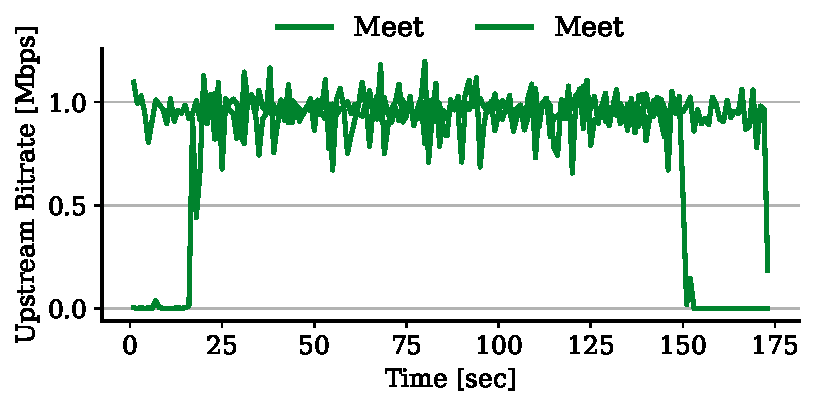
\includegraphics[width=1\textwidth]{figures/appendix/meet_meet_3_ul_r2.pdf}
    \caption{Meet vs. Meet}
    \label{subfig:meet-meet-3}
\end{subfigure}\hfill
\begin{subfigure}[t]{.4\textwidth}
    \centering
    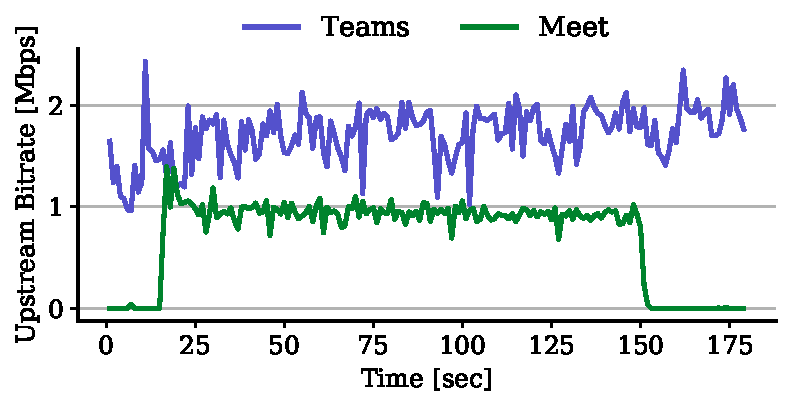
\includegraphics[width=1\textwidth]{figures/appendix/teams_meet_3_ul_r3.pdf}
    \caption{Teams vs. Meet}
    \label{subfig:teams-meet-3}
\end{subfigure}
\begin{subfigure}[t]{.4\textwidth}
    \centering
    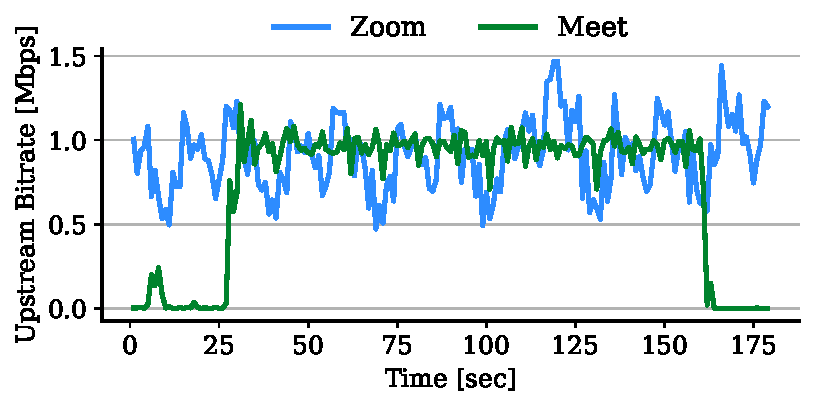
\includegraphics[width=1\textwidth]{figures/appendix/zoom_meet_3_ul_r2.pdf}
    \caption{Zoom vs. Meet}
    \label{subfig:zoom-meet-3}
\end{subfigure}
\begin{subfigure}[t]{.4\textwidth}
    \centering
    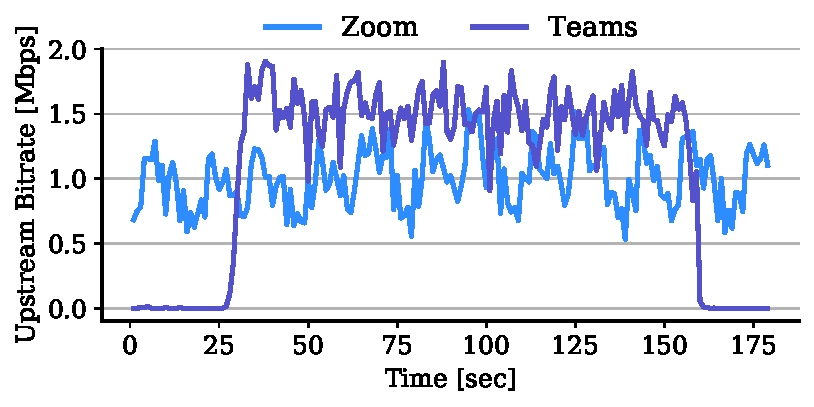
\includegraphics[width=1\textwidth]{figures/appendix/zoom_teams_3_ul_r2.pdf}
    \caption{Zoom vs. Teams}
    \label{subfig:zoom-teams-3}
\end{subfigure}
\begin{subfigure}[t]{.4\textwidth}
    \centering
    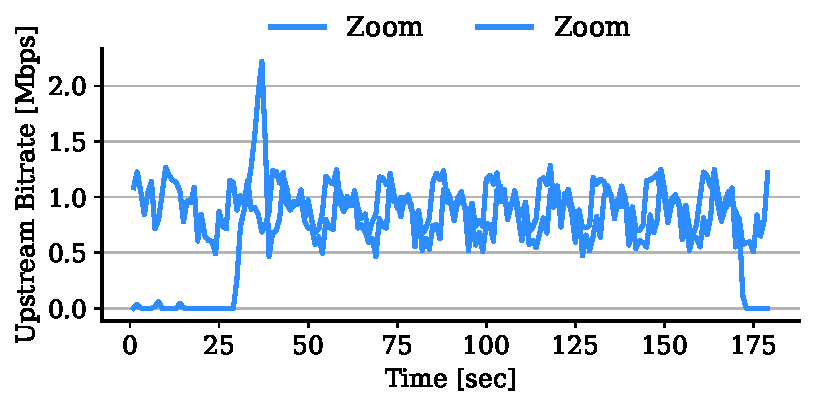
\includegraphics[width=1\textwidth]{figures/appendix/zoom_zoom_3_ul_r1.pdf}
    \caption{Zoom vs. Zoom}
    \label{subfig:zoom-zoom-3}
\end{subfigure}
\caption{VCA vs. VCA on a 3 Mbps symmetric connection.}
\label{fig:vca-vca-3}
\end{figure}

\section{Static Experiments - Repetition on Mac Operating System (MACOS)}
\label{appendix:static}
Here, we demonstrate the extensibility of our automation framework for macOS. More specifically, we repeat the experiments from Section~\ref{sec:static} with the uplink shaped on a device running macOS. We use a 2017 MacBook Air with 8GB 1600 Mhz DDR3 memory, 1.8 GHz Dual-Core Intel Core i5 processor, and Intel HD Graphics 6000 1536 MB Graphics. The laptop is running macOS Version 10.15.7. The MacBook Air initiates a call with a Linux client with the same specifications as outlined in Section 2.2. We use Zoom Version 5.7.6 and Chrome Version 92.0.4515.159. We test the
browser version of Teams and the native client of Zoom and Meet. 

We did find some platform-specific differences. The macOS does not support v4l2loopback; instead we use Open Broadcaster Software or OBS (Version 27.0.1) to feed in the same
talking-head video used throughout our experiments. In addition, we only include the \teamsbrowser client for Teams and omit the native client. This is because the current version of the Teams client on macOS does not support virtual camera~\cite{teams_virtual_camera}. 


\begin{comment}
\begin{table}[]
\begin{tabular}{|c|c|c|}
\hline
\multirow{2}{*}{\textbf{VCA}} & \multicolumn{2}{c|}{\textbf{Utilization (Mbps)}} \\ \cline{2-3} 
                              & Upstream               & Downstream              \\ \hline
Meet                          & 0.89                   & 0.83                    \\ \hline
Teams                         & -                      & 1.43                    \\ \hline
Zoom                          & 0.96                   & 0.88                    \\ \hline
\end{tabular}
\caption{Unconstrained network utilization on macOS}
\label{tab:vca_static_mac}
\end{table}
\end{comment}

\textbf{Results}: 
Figure~\ref{fig:uplink_static_mac} shows the uplink network utilization on the macOS device. The overall trends are similar as on Linux (see Figure 
~\ref{subfig:uplink_bitrate}). We do find few differences between the two platforms: % Looking first at Figure ~\ref{subfig:vca_static_mac}, the VCAs follow similar trends as in Figure 
%~\ref{subfig:uplink_bitrate},
\zoom has a higher nominal utilization on macOS ($0.96$ Mbps) than Ubuntu ($0.78$ Mbps). \meet has a 
slightly lower uplink utilization, using $0.89$ Mbps on Mac and $0.95$ Mbps on Ubuntu. Finally, \teamsbrowser has a higher
nominal utilization on macOS than Ubuntu. Some of these differences could be due to updated VCA version itself, while others could be attributed to the differences in the operating system. 


We next report application performance metrics by logging the WebRTC stats API as in Section~\ref{subsec:application_performance}. We find that \meet adapts to the constrained throughput setting mainly by increasing the quantization parameter. On the other hand, \teamsbrowser simultaneously adapts both the sent frames per second and the quantization parameter of the encoded video. Interestingly, there are some minor differences compared to Ubuntu. For instance, the sent frame width for \meet does not change on macOS at low capacity region (0.3-0.5 Mbps), while it decreased in the case of Ubuntu. This is despite the fact that the browser-based \meet can ideally use similar codebase across operating systems. However, with the current experiment setup, it is not clear if the root cause of the difference can be attributed to the operating system. This is because \meet may have updated in between the two set of experiments were conducted. In future work, we plan to repeat the experiments around similar time to understand any operating system-specific differences. 

\begin{figure}[]
%\begin{subfigure}[t]{0.4\textwidth}
    \centering
    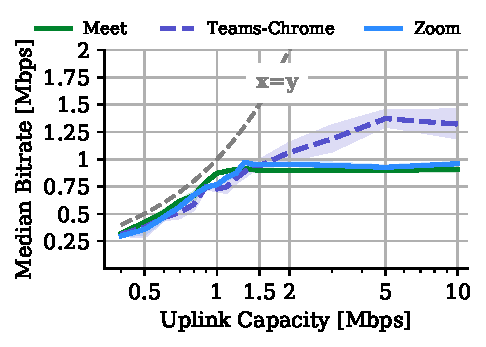
\includegraphics[width=0.4\textwidth,keepaspectratio]{figures/static_mac/uplink_mac.pdf}
    %\caption{Uplink bandwidth vs network bitrate}
	%\label{subfig:uplink_bitrate_mac}
%\end{subfigure}\hfill
\caption{Uplink network utilization under different shaping levels. The bands represent 90\% confidence intervals.}
\label{fig:uplink_static_mac}
\end{figure}


\begin{figure*}[t]
        \begin{subfigure}[t]{0.33\textwidth}
    		\centering
        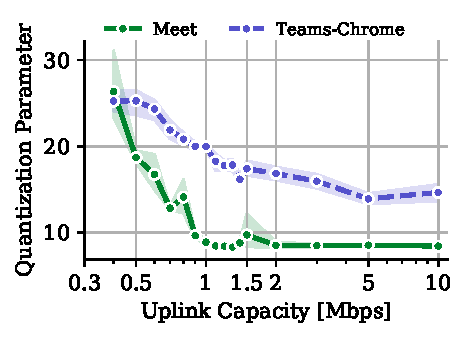
\includegraphics[width=\textwidth,keepaspectratio]{static_mac/uplink_s_qpsum_mac.pdf}
        \caption{Uplink - Quantization parameter.}
 		\label{subfig:uplink_video_qp_mac}
    \end{subfigure}%
    \hfill
	\begin{subfigure}[t]{0.33\textwidth}
        \centering
        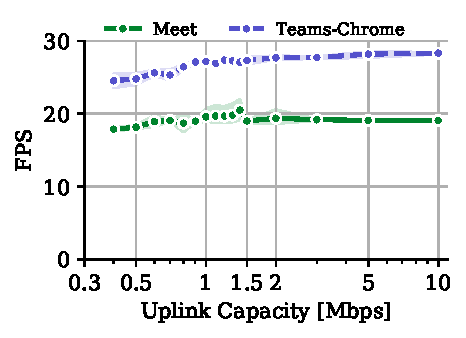
\includegraphics[width=\textwidth]{static_mac/uplink_sent_framesPerSecond_mac.pdf}
    \caption{Uplink - Frames per second.}
    \label{subfig:uplink_frames_per_second_mac}
    \end{subfigure}% 
    \hfill
	\begin{subfigure}[t]{0.33\textwidth}   
        \centering
        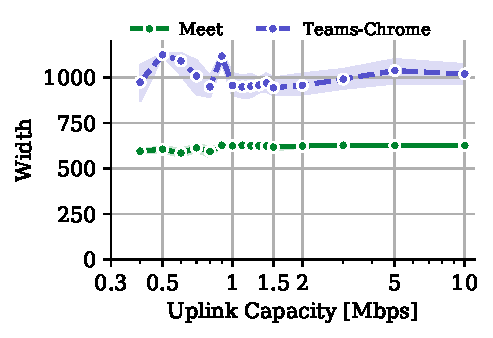
\includegraphics[width=\textwidth]{static_mac/uplink_sent_frameWidth_mac.pdf}
    \caption{Uplink - Frame width.}
    \label{subfig:uplink_frame_width_mac}
    \end{subfigure}
	\caption{Video encoding parameters with 90\% confidence intervals under upstream throughput constraints.}
    \vspace{-1em}
	\label{fig:video_qual}
\end{figure*}




\begin{comment}
\begin{subfigure}[t]{0.4\textwidth}
    \centering
    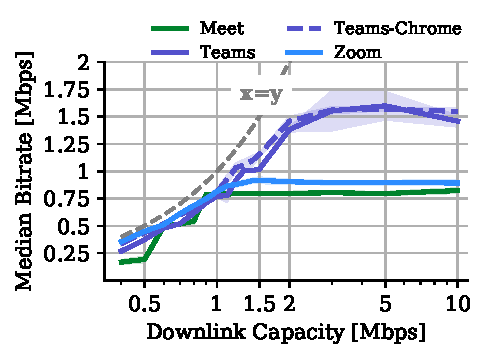
\includegraphics[width=\textwidth,keepaspectratio]{figures/static_mac/downlink_mac.pdf}
    \caption{Downlink bandwidth vs network bitrate}
	\label{subfig:downlink_bitrate_mac}
\end{subfigure}
\end{comment}

\begin{comment}
\begin{subfigure}[t]{0.33\textwidth}
		\centering
    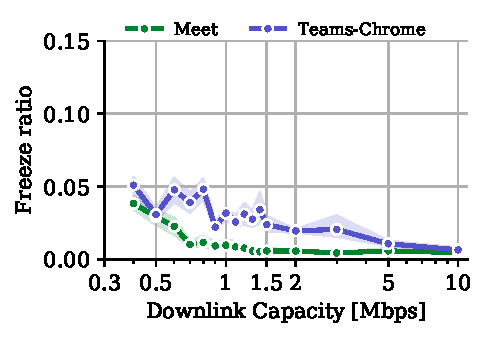
\includegraphics[width=\textwidth,keepaspectratio]{figures/static_mac/downlink_freezeRatio_mac.pdf}
    \caption{Downlink - Freeze Ratio}
 	\label{subfig:downlink_video_qp_mac}
\end{subfigure}%
\hfill
\begin{subfigure}[t]{0.33\textwidth}
    \centering
    \includegraphics[width=\textwidth]{static_mac/downlink_received_framesPerSecond_mac.pdf}
\caption{Downlink - Frames per second.}
\label{subfig:downlink_frames_per_second_mac}
\end{subfigure}% 
\hfill
\begin{subfigure}[t]{0.33\textwidth}
    \centering
    \includegraphics[width=\textwidth]{static_mac/downlink_received_frameWidth_mac.pdf}
\caption{Downlink - Frame width.}
\label{subfig:downlink_frame_width_mac}
\end{subfigure}
\newline
\end{comment}


\end{sloppypar}
\end{document}

%%%%%%%%%%%%%%%%%%%%  END OF DOCUMENT  %%%%%%%%%%%%%%%%%%%%
